\chapter[Preprocessing of time series]{Compression and classification with Dynamic Time Warping}
\label{fdtw}
%\minitoc

\begin{abstract}
 Dynamic Time Warping (DTW) is a time series alignment algorithm that is often used because it
 considers that it exits small distortions between time series during their alignment.  However, DTW
 sometimes produces pathological alignments that occur when, during the comparison of two time series
 X and Y, one data point of the time series X is compared to a large subsequence of data points of Y.
 In this chapter, we demonstrate that  compressing time series using Piecewise Aggregate Approximation
 (PAA) is a simple strategy that greatly increases the quality of the alignment with DTW. This result is 
 particularly true for synthetic data sets.      
 \end{abstract}

\section{Introduction}
%


Time series databases are often large and several transformations have been
introduced in order to represent them in a more compact way. One of these transformations is
Piecewise Aggregate Approximation (PAA) \cite{keogh2001dimensionality}, which consists in dividing a
time series into several segments of fixed length and replacing the data points of each segment with
their averages. Due to its simplicity and low computational time, PAA has been widely used as a
basic primitive by other temporal data mining algorithms such as SAX \cite{lin2003symbolic}, SAX-TD \cite{sun2014improvement}, ESAX  \cite{lkhagva2006extended}, in order to: 
\begin{itemize}
  \item Construct symbolic representations of time
series; \cite{camerra2010isax} \\ \cite{ulanova2015scalable}.
  \item Construct an index for time series; \cite{zhao2016shapedtw} \\ \cite{keogh2000scaling}  \cite{Kate2016}. Indeed, PAA allows queries, which are shorter than length for which the
index was built. This very desirable feature is impossible with Discrete Fourier Transform, Singular
Value Decomposition and Discrete Wavelet Transform.
\item Classify time series.
\end{itemize}


\subsection{PAA and Dynamic Time Warping}

 Time series comparison is an important task that
can be done in two main ways.
Either the comparison method  considers that there is no time distortion as in Euclidian distance
(ED), or it considers that  some small time distortions  exist between time axis of time series as
in Dynamic Time Warping alignment algorithm (DTW)
\cite{Zhang_Tang_Duan_2015}. Since time distortion often exists between time series, DTW  has often
better results than ED \cite{UCRArchive}. An exhaustive comparison of time series algorithms
\cite{Bagnall} showed that DTW is among the efficient techniques to be used. However, DTW has two major
drawbacks:
 the comparison of two time series with this algorithm is time-consuming
\cite{Rakthanmanon_Campana_Mueen_Batista_Westover_Zhu_Zakaria_Keogh_2012} and sometimes DTW
 produces pathological alignments \cite{Keogh_Pazzani_2001}. A
pathological alignment occurs when, during the comparison of two time  series $X$
and $Y$, one datapoint of the time series $X$ is compared to a large subsequence
of datapoints of $Y$;  A pathological alignment causes a wrong comparison.


 Three categories of methods are used to avoid pathological alignments with DTW:

\begin{itemize}
  \item The first one adds constraints to DTW \cite{Ratanamahatana_Keogh_2004} \cite{Yu_Yu_Hu_Liu_Wu_2011}  \cite{candan2012sdtw}  \cite{sakoe1978dynamic} \\ \cite{jeong2011weighted}  \cite{salvador2007toward}.
  The main idea of these methods is to limit the length of the subsequence of a time series
  that can be compared to a single datapoint of another time series.
  
  \item The second one suggests skipping data points that
  produce pathological alignment during the comparison of two time series \cite{longin2005elastic} \\ \cite{itakura1975minimum}  \cite{myers1980performance}.
  \item The third one proposes to replace the datapoints of time
  series with a high-level abstraction that captures the local behavior of those
  time series. A high-level abstraction can be a histogram of values that
  captures the distribution of time series datapoints in space \cite{Zhang_Tang_Duan_2015} or a 
  feature that captures the local  properties of time series, such as the trend with Derivative DTW
  (DDTW) \cite{Keogh_Pazzani_2001}.
\end{itemize}
Another simple but yet interesting way to capture local properties of time series is to  consider the mean of segments of the time series as PAA does. Indeed, the use of the mean reduces the harmful effects of singularities contained in the data and thus allows to avoid pathological
alignments.  However, one major challenge with PAA is the choice of the number of segments to
consider especially with long time series.


\subsection{Choise of a segment number with PAA}

If the number of segments considered with PAA is too small, the resulting
representation  is compact, but it contains less information. On the other hand, if the number of
segments is too large, the obtained representation  is less compact and more prone to the noise
contained in the original time series (Fig. \ref{relation_nb_acc}). Our idea is that a number of
segments for PAA will be considered as good (1) if it allows obtaining a compact representation of the
time series, and (2) if it preserves the quality of the alignment of time series. So when
considering classification task, one of the best algorithm to use for
evaluating the quality of time series alignment is one Nearest Neighbor (1NN).   
Indeed, its classification error directly depends on time series alignment, since 1NN has no other
parameters \cite{wang2013experimental}.


\begin{figure}
\center
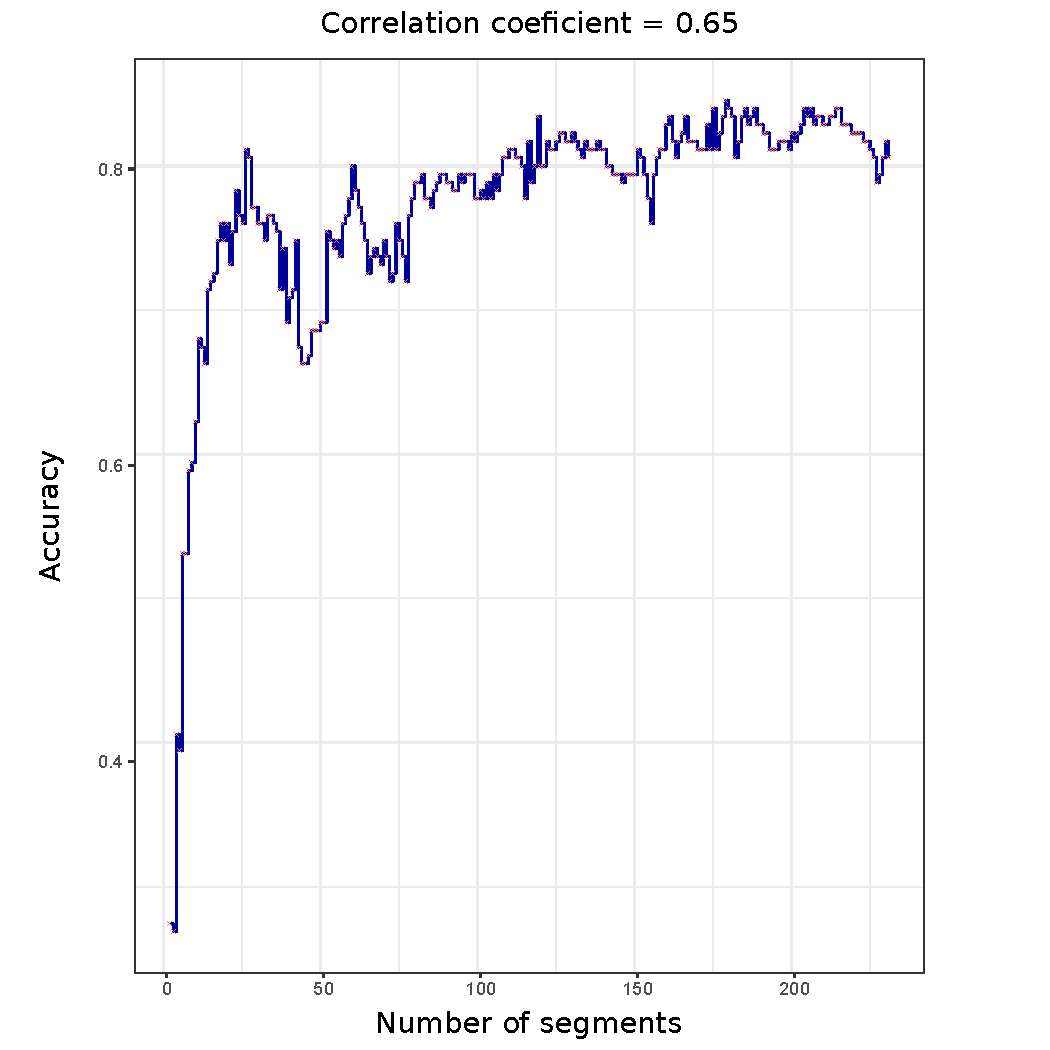
\includegraphics[scale = 0.4]{effets_de_n_sur_accuracy}
\caption{Relation between Accuracy and the number of segment on FISH dataset. The accuracy is computed from the algorithm one nearest neighbor (1NN) associated with PDTW. When the number of segments
considered is very small (bellow 20), there is a loss of information and the accuracy is reduced. However, considering all the points in the time series, do not produce a maximum accuracy due to the presence of noise or singularities \cite{Keogh_Pazzani_2001}  in the data. }
\label{relation_nb_acc}
\end{figure}

\subsection{Summary of Contributions}

In this chapter, 
\begin{itemize}
\item We define the problem of preprocessing time series with PAA for a better classification with
DTW;
\item We propose a parameter free heuristic for aligning piecewise aggregate time series with DTW, which approximates the optimal value of the number of segments to be considered with PAA. 
\end{itemize}

The rest of the chapter is organized as follows: in Section
\ref{sec:1} we recall the definitions and background; Section \ref{sec:3} explains our approach;
Section \ref{sec:4} presents experimental results and comparisons to other methods; Section
\ref{sec:5} draws conclusions and venues for future work.   




\section{Background and related works}
\label{sec:1}
Let's recall some definitions \ref{siyouRairo}.

\begin{definition}
A \textbf{time series}
$X=x_{1},\cdots,x_{n}$ is a sequence of numerical values representing the evolution of a specific quantity over time. $x_{n}$ is the most recent value.
\end{definition}

\begin{definition}
A segment  $X_{i}$ of length  $l$ of the time series $X$ of length $n$
$(l<n)$ is a sequence constituted by $l$ \hyphenation{conse-cutive} variables of $X$ starting at the position $i$ and ending at the position $i+l-1$.
We have: $X_{i}=x_{i},x_{i+1},...,x_{i+l-1}$.
\end{definition}

\begin{definition}
The arithmetic average of the data points of a segment  $X_{i}$ of length
$l$ is noted $\bar{X}_{i}$ and is defined by:
\begin{eqnarray}
\bar{X}_{i}=\frac{1}{l}\sum_{j=0}^{l-1}x_{i+j}.
\end{eqnarray}
\end{definition}


\begin{definition}

Let $T$ be the set of time series. The Piecewise Aggregate Approximation (PAA) is defined as follows:

\begin{eqnarray}
\begin{array}{ccc}
 PAA: T\times\mathbb{N^{*}}\rightarrow T\\
\\
(X,N)\mapsto PAA(X,N) & = &
 \begin{cases}
 \begin{array}{c}
\bar{X}_{k}, k \in \{i\times\frac{n}{N} + 1, i=0,\cdots , N-1\}\;if\:N<|X|\\
X\:otherwise
\end{array}
\end{cases}
\end{array}
\end{eqnarray}

\end{definition}

\begin{definition}
Let $d\subseteq T$ be a subset of time series,
$N\in\mathbb{N}^{*},\:PAAset(d,N)=\{PAA(X,N),\:\forall X\in d\}.$
\end{definition}

\subsection{Dynamic Time Warping algorithm.}
DTW \cite{sakoe1978dynamic} is an algorithm of time series alignment
algorithm that  performs a non-linear alignment while
minimizing the distance between two time series. To align two time series: 
$X=x_{1},x_{2},\cdots,x_{n};\,
Y=y_{1},y_{2},\cdots,y_{m},$ the algorithm constructs an  $n\times m$  matrix where the cell $(i,
j)$ of the matrix corresponds to the squared distance $(x_{i}-y_{j})^{2}$ between $x_{i}$
and $y_{j}$. Then to find the best alignment between $X$ and $Y$, DTW constructs the path that minimizes the sum of squared distances. This path, noted
$W = w_1, w_2, \ldots, w_k, \ldots, w_K,$ must respect the following constraints:
\begin{itemize}
  \item Boundary constraint: $w_1 = (1, 1)$ and  $w_K = (n, m)$;
  \item Monotonicity constraint: given $w_k = (i, j)$ and :  $w_{k + 1} =
  (i',j')$ then: $i \leq i'$ and $j \leq j'$;
 \item Continuity constraint: given $w_k = (i, j)$ and:   $w_{k + 1} = (i', j')$
 then: $i' \leq i + 1$ and: $j' \leq j + 1$.
\end{itemize}
The warping path is computed by  an algorithm based on the dynamic
programming paradigm that solves the following recurrence:
\begin{eqnarray}
\begin{array}{l}
\gamma(i,j)=d(x_{i},y_{j}) + min\{\gamma(i-1, j-1), \\
\gamma(i-1, j),\gamma(i, j-1)\},
\end{array}
\end{eqnarray}


where $d(x_{i},y_{j})$ is the squared distance contained in the cell $(i, j)$ and $\gamma(i, j)$ is the cumulative distance at the position $(i, j)$ that is computed by the sum of the squared distance at the position $(i, j)$ and the minimal cumulative distance of its three adjacent cells.


Piecewise Dynamic Time Warping Algorithm (PDTW) \cite{keogh2000scaling} is the DTW algorithm applied on Piecewise Aggregate time series \cite{keogh2001dimensionality}. Let $N\in\mathbb{N^{*}}$, $X$ and $Y$ be two time series:
\begin{eqnarray}
PDTW(X, Y, N) = DTW(PAA(X, N), PAA(Y, N)).
\end{eqnarray}

The number  of segments $N$ that one considers greatly influences the quality of the alignment of the time series. However, PDTW does not give any information on the way to choose it. For making this choice, \cite{chu2002iterative} proposes the Iterative Deepening Dynamic Time Warping Algorithm (IDDTW).



\subsection{Iterative Deepening Dynamic Time Warping}
\label{sec:2}

For determining the number of segments, IDDTW only considers values that are  power of 2 and for each value, computes an error distribution by comparing PDTW with the standard DTW at each level of compression. It takes as inputs: the query $Q$, the dataset $D$, the user's confidence (or tolerance for false dismissals) $user\_conf$ , and the set of standard deviations $StdDev$ obtained from the error distribution. Example: Let $C$ and $Q$ be two time series of the dataset $D$, let $best\_so\_far$ be the $DTW$ distance between two time series of the dataset. Suppose the distance $D_{pdtw}(Q, D)$ is 40 and the $best\_so\_far$ is $30$. The difference between the estimated distance and the $best\_so\_far$ is $10$. Using the error distribution centred around the approximation $(40)$, we can determine the probability that the candidate could be better by examining the area beyond the location of the $best\_so\_far$ (shown in solid black in
Figure \ref{iddtwPrinciple}): We disqualify a candidate if this probability is less than the user's specified error acceptance, the candidate is disqualified; otherwise, a finer aproximation is used and the test is re-applied to the next depth. This process continues until the full DTW is performed.


\begin{figure}
\center
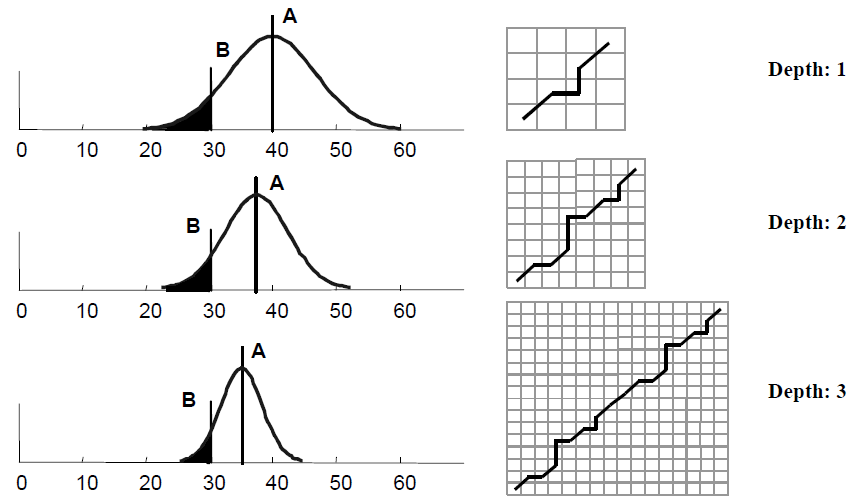
\includegraphics[scale=0.4]{iddtw}
\caption{IDDTW operating principle. Depth represents approximation levels, A represents approximate distance and B is best\_so\_far \cite{chu2002iterative}. }

\label{iddtwPrinciple}

\end{figure}

More precisely, IDDTW proceeds as follows: 

\begin{itemize}
  \item the algorithm starts by applying the classic DTW  to the first $K$ candidates from the dataset. The results of the best matches to the query are contained in $R$, with $|R|=K$. The $best\_so\_far$ is determined from $argmax{R}$;

\item both the query $Q$ and each subsequent candidate $C$ are approximated using PAA representations with  $N$  segments to determine the corresponding PDTW;

\item a test is performed to determine whether the candidate $C$ can be pruned off or not. If the result of the test is found to have a
probability that it could be a better match than the current $best\_so\_far$, a higher resolution of the approximation is required. Then each segment of the candidate is split into two segments to obtain a new candidate;

\item the process of approximating $Q$ and $C$ to determine the PDTW
should be reapplied and the test is repeated for all approximations levels until they fail the test or their true distance DTW is determined.
\end{itemize}

In this way, IDDTW finds the number of segments that best approximates DTW and speeds up its computation. However, IDDTW has three main limitations:

\begin{itemize}
  \item it only considers the numbers of segments for PDTW that are
  power of 2;
  \item it requires a user-specified tolerance for false dismissals
  that influences the quality of the approximation, but the algorithm does not give any indication on how to choose the tolerance;
  \item it considers DTW as a reference while looking for the  number of segments that best aligns the time series. However, because of pathological alignments, DTW sometimes fails to align time series properly \cite{Keogh_Pazzani_2001}.
\end{itemize}


 Our goal is to find the number of segments that best aligns the time series and also speeds up the computation of DTW.



\section{FDTW: a GRASP based heuristic}
\label{sec:3}

We propose a  heuristic named parameter Free piecewise DTW (FDTW) based on Greedy Randomized Adapted Search Procedure that deals with all the limitations of IDDTW: it considers all the possible values for the number of segments, it is parameter-free and it finds a number of segments for PDTW based on the quality of  the time series alignment, namely the error rate for classification task. The next section introduces FDTW.

\subsection{ Evaluation procedures for the compression quality}
Before explaining how to evaluate the quality of time series compression, we
first describe the time series datasets that we considered. They are
made up of time series associated with labels that identify their shapes. For instance, in the ECG dataset, each time series traces the
electrical activity recorded during one heartbeat. These time series are split in two classes: normal heartbeat and myocardial infarction. 

 Time series classification is a classic problem, which consists in guessing the label of an unlabeled time series  based on its shape.
The quality of a time series classification model is evaluated from its classification error ($\epsilon$), or its accuracy ($a = 1 - \epsilon$).  When considering a classification task, one of the
best classification algorithm  for evaluating the quality of time series
alignment is \textbf{one Nearest Neighbor (1NN)}. Indeed,  its classification
error directly depends on time series alignment, since 1NN has no other parameters \cite{wang2013experimental}.

During this work, a compact representation of time series  is considered to be good
if it reduces the length of the original time series, but also if the classification error
obtained by classifying the compact time series is small. The classification error is small
when the time series keep their characteristic shape despite compression.   



\subsection{Problem definition.}

Let $D = \{d_i\}$ be a set of datasets composed of time series. We note
$|d_i|$ the number of time series of the dataset $d_i$.

Let $X \in d_i$ be a time series of the dataset $d_i$; we note $|X| = n$ the length of the time series $X$. For simplicity of notation we suppose that all the time series of $d_i$ have the same length.

\begin{definition}
\begin{eqnarray}
 1NNDTW: D \rightarrow [0, 1] \\
  d_i\mapsto 1NNDTW(d_i)
\end{eqnarray}


 $1NNDTW(d_i)$ is the classification error of one Nearest Neighbour with Dynamic Time Warping on the dataset $d_i$.
\end{definition}




\begin{definition}
\begin{eqnarray}
\begin{array}{l}
 1NNPDTW: D\times\{1 \ldots n\}\rightarrow [0, 1]\\
 \\
(d_i, N)\mapsto 1NNPDTW(d_i, N) \\
 =  1NNDTW \circ PAAset ( d_i, N) 
\end{array}
\end{eqnarray}
\end{definition}

$1NNPDTW( d_i, N)$  is the classification error of 1-NN with PDTW using $N$ segments on 
 $d_i$.

\paragraph{}Our goal is to find the number of segments that allows $PDTW$ to best align
time series.  $PDTW$ gives a good alignment when its
classification error with $1NN$ is low
\cite{Rakthanmanon_Campana_Mueen_Batista_Westover_Zhu_Zakaria_Keogh_2012}.  Our
problem is then to find the number of segments $N$ that minimizes $1NNPDTW(d_i,
N)$.

Formally, \textbf{ given a dataset $d_i,$ of time series that have a length n, we look for the number
of segments $N \in \{1 \ldots n \}$ such that}

\begin{eqnarray}
\underset{1\leq N\leq n}{min}\{1NNPDTW(d_i,N)\}.
\end{eqnarray}


\subsection{Brute-force search.}

The simplest way to find the value for the number of segments that minimized the
classification error is to test all the possible values.  Obviously, this
method is time consuming as it requires to test $n$ values to find the best one. The time complexity is:
\begin{eqnarray}
O(|d|^{2} \times n^{3}),
\end{eqnarray}

where $C$ is the set of values for the number of segments.

To reduce the time of the search,  FDTW proposes to look for the
number of segments with the minimal classification error without testing all the possible values.

\subsection{ Greedy Randomized Adaptive Search Procedures}
The Greedy Randomized Adaptive Search Procedures (GRASP) is a multi-start, or iterative metaheuristic proposed by Feo and Resende
(1995) \cite{feo1995greedy}, in which each iteration consists of two phases:
firstly a new solution is constructed by a greedy randomized
procedure and this solution is then improved using a local search procedure.


The greediness criterion establishes that candidates with the best quality are
 added to a restricted list of candidates. Then, one of the candidate of the restricted list is  chosen at random when
building up the solution. The candidates obtained by greedy algorithms are not
necessarily optimal, but they are used as initial solutions
to be explored by local search. The heuristic  we proposed is build upon
GRASP and strengthened with an inclusion of specific global search component.




\subsection{Parameter free heuristic}
The idea of our heuristic is the following:
\paragraph{1.} We choose $N_{c}$ candidates number of segments, distributed in the space of possible values
to ensure that we are going to have small, medium and large values as
candidates. The candidates values are: $n,\,n-\left\lfloor
\frac{n}{N_{c}}\right\rfloor ,\,n-2\times\left\lfloor \frac{n}{N_{c}}\right\rfloor
,\,...,\,n-N_{c}\times\left\lfloor \frac{n}{N_{c}}\right\rfloor $. For instance, if the length of
time series is $n = 12$ and the number of candidates is $N_c = 4$, we are going to select the
candidates 12, 9, 6, 3.

\begin{center}
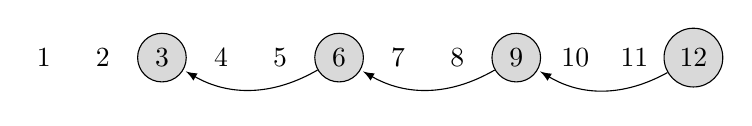
\begin{tikzpicture}[shorten >=1pt,->]

\node (1) at (1,1) {1};
\node (2) at (1.75,1) {2};
\node[draw,circle,fill=gray!30] (3) at (2.5,1) {3};
\node (4) at (3.25,1) {4};
\node (5) at (4,1) {5};
\node[draw,circle,fill=gray!30] (6) at (4.75,1) {6};
\node (7) at (5.5,1) {7};
\node (8) at (6.25,1) {8};
\node[draw,circle,fill=gray!30] (9) at (7,1) {9};
\node (10) at (7.75,1) {10};
\node (11) at (8.5,1) {11};
\node[draw,circle,fill=gray!30] (12) at (9.25,1) {12};

\draw[->,>=latex] (12) to[bend left] (9);
\draw[->,>=latex] (9) to[bend left] (6);
\draw[->,>=latex] (6) to[bend left] (3);

\end{tikzpicture}
\end{center}



\paragraph{2.} We evaluate the classification error with $1NNPDTW$ for each chosen candidate, and we
select the candidate that has the minimal classification error: it is the best candidate.
In our example, let us suppose that we get the minimal value with the candidate 6: it is thus the
best candidate at this step.

\begin{center}
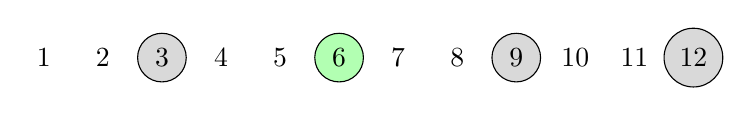
\begin{tikzpicture}[shorten >=1pt,->]

\node (1) at (1,1) {1};
\node (2) at (1.75,1) {2};
\node[draw,circle,fill=gray!30] (3) at (2.5,1) {3};
\node (4) at (3.25,1) {4};
\node (5) at (4,1) {5};
\node[draw,circle,fill=green!30] (6) at (4.75,1) {6};
\node (7) at (5.5,1) {7};
\node (8) at (6.25,1) {8};
\node[draw,circle,fill=gray!30] (9) at (7,1) {9};
\node (10) at (7.75,1) {10};
\node (11) at (8.5,1) {11};
\node[draw,circle,fill=gray!30] (12) at (9.25,1) {12};

\end{tikzpicture}
\end{center}

\paragraph{3.} We respectively look between the predecessor (i.e., 3 here) and successor (i.e., 9
here) of the best candidate for a number of segments with a lower classification error: this number
of segments corresponds to a local minimum.
In our example, we are going to test values 4, 5, 7 and 8 to see if there is a local minimum.

\begin{center}
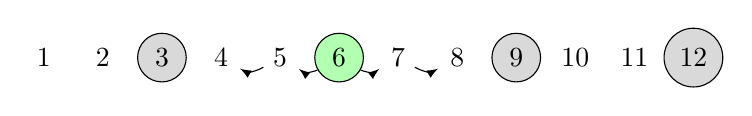
\begin{tikzpicture}[shorten >=1pt,->]

\node (1) at (1,1) {1};
\node (2) at (1.75,1) {2};
\node[draw,circle,fill=gray!30] (3) at (2.5,1) {3};
\node (4) at (3.25,1) {4};
\node (5) at (4,1) {5};
\node[draw,circle,fill=green!30] (6) at (4.75,1) {6};
\node (7) at (5.5,1) {7};
\node (8) at (6.25,1) {8};
\node[draw,circle,fill=gray!30] (9) at (7,1) {9};
\node (10) at (7.75,1) {10};
\node (11) at (8.5,1) {11};
\node[draw,circle,fill=gray!30] (12) at (9.25,1) {12};

\draw[->,>=latex] (6) to[bend left] (5);
\draw[->,>=latex] (5) to[bend left] (4);
\draw[->,>=latex] (6) to[bend right] (7);
\draw[->,>=latex] (7) to[bend right] (8);

\end{tikzpicture}
\end{center}
\paragraph{4.} We restart at step one while choosing
different candidates during each iteration to ensure that we return a good
local minimum. We fix the number of iterations to $k \leq \left\lfloor log(n)\right\rfloor $. At each iteration, the first candidate is $n-(number \_ of \_ iteration \,-\, 1)$.


\paragraph{}In short, in the worst case, we test the first $M$ candidates to find the best one.
Then, we test $\frac{2n}{M}$ other candidates to find the local minimum.
We finally perform $nb(M)\, =\, M\, +\, \frac{2n}{M}$ tests. The number of tests
 to be performed is a function of the number of candidates. Hence, how many
candidates should we consider to reduce the number of tests? The first
derivative of $nb$ function  vanishes when $M=\sqrt{2n}$ and its second derivative is
positive; so the minimal number of tests is obtained when the number of candidates is : 
$M=\sqrt{2n}$. At each
iteration, the heuristic tests $nb(\sqrt{2n})=\sqrt{8n}$ number of segments. As we have $k$
iterations the number of candidates tested is: $|C|=k\sqrt{8n}$. The details of the heuristic are presented in Algorithm \ref{algo5}.

\paragraph{Time complexity: }
We use the training set to find the number of segments that should be considered
with PDTW. For that purpose, we applied $1NN$ on the training set that costs
\begin{eqnarray}
O(|d|^{2} \times n^{2}\sqrt{n}).
\end{eqnarray}


where $|d|^{2}$ comes from $1NN$ algorithm and
$n^{2}\sqrt{n}$ comes from $PDTW$. 



\paragraph{}\textbf{Lemma 1: } \\
For a given dataset $d_i$, the quality of the alignment of our heuristic
is better than that of DTW: $ FDTW(d_{i}) \leq 1NNDTW(d_{i}) $.


\paragraph{}\textbf{Proof: } \\
 $1NNDTW(d_i) = 1NNPDTW(d_i,n)$. Then, $1NNDTW(d_i)$ is one of the
candidates considered by the heuristic $FDTW$. Since $FDTW$ returns the
minimal classification error from all candidates, the classification error of
$1NNDTW$ is always greater than or equal to $FDTW$.



\begin{algorithm}[h]
\DontPrintSemicolon
\KwIn{training\_set, length of a time serie : n, \\ number of iterations :
nb\_rep}
\KwOut{The number of segments to be used N \\ The accuracy associated to N}
\SetKwBlock{Begin}{function}{end function}

\Begin($\text{FDTW} {(} training\_set, n, nb\_rep {)}$)
{
  $l \leftarrow floor(n/sqrt(2 * n))$\;
  $tab\_N \leftarrow ones(n)$\;
  \ForAll{$i \in \left\lbrace  0, 1, \ldots, (nb\_rep - 1)\right\rbrace$}
  {
    $tab\_N\_possible\_candidates \leftarrow seq(from = (n - i), to = 1, by = -l)$\;
    $nb\_candidats \leftarrow |tab\_N\_possible\_candidates|$\;

    \For{$i \;in\left\lbrace 1, 2, \ldots, nb\_candidates\right\rbrace $}
    {
      \uIf{$tab\_N[tab\_N\_possible\_candidates[i]] \; \neq  \;0$}
      {
       $tab\_N\_candidates[j] \leftarrow tab\_N\_possible\_candidates[i] $\;
       $tab\_N[ tab\_N\_candidates[j] ] \leftarrow 0 $\;
       $j \leftarrow j + 1$
      }

    }
    $mat\_r \leftarrow 1NNPDTW(training\_set, tab\_N\_candidats)$ \;\tcc{$1NNPDTW$ return a matrix of couple $(N,error)$}

    $min \leftarrow minimun(mat\_r) $\;\tcc{$minimum$ return the couple $(N,error)$ with the minimum error}
    $result[(i + 1)]   \leftarrow localMinimun(min.N,  min.error, training\_set,
    tab\_N)$\;
      
  }
  $m \leftarrow minimun(result)$\;
    
  \Return{$m$}

}
\caption{Parameter Free Dynamic Time Warping}\label{algo5}
\end{algorithm}


\paragraph{}Nevertheless, a heuristic does not always give the optimal value. To ensure that
it gives a result not far from the optimal value, one approach is to
 guarantee that the result of the heuristic always lies within an interval with respect to the optimal
value \cite{ibarra1975fast}.

In our case, we are looking for the number of segments that allows a good
alignment of time series. The alignment is good when the classification error
with 1NN is minimal or when the accuracy is maximal.

Let $d_i$ be a dataset: 

$acc_{max(d_i)} = 1-\underset{1\leq\alpha\leq
n}{min}\{1NNPDTW(di,\alpha)\}$ is the maximal accuracy for the dataset $d_i$,

$acc_{DTW} = 1 - 1NNDTW(d_i)$ is the accuracy obtained with $d_i$ and 1NNDTW, and


$acc_{FDTW}=1 - FDTW(d_i)$ is the accuracy of our heuristic.

To ensure the quality of our heuristic FDTW, we hypothesized that $1NNDTW$ is better than
Zero Rule classifier. Zero Rule classifier is a simple classifier that predicts the majority class of test data (if nominal) or average value (if numeric). Zero Rule is often
used as baseline classifier \cite{cuvrin2007meeting}. The minimal value of the
accuracy of Zero Rule is $\frac{1}{c}$ where c is the number of classes of the
dataset.

\paragraph{}\textbf{Proposition 1.:}\\
For a given dataset $d_i$ that has $c_i$ classes, $c_i\in \mathbb{N}^*,$

$
if \; acc_{DTW} \geq \frac{1}{c_i} \; then \;  \frac{1}{c_i} \times acc_{max}
\leq acc_{FDTW} \leq acc_{max}
$

Proposition 1 shows that  1NN associated with DTW has a better accuracy than the baseline
classifier Zero Rule; the FDTW heuristic is a parametric approximation.

\paragraph{}\textbf{Proof: }\\
By definition, $ acc_{FDTW} \leq acc_{max}$ 
We look for $\beta \in \mathbb{N}$ such that 

\begin{eqnarray}
\frac{1}{\beta}\times acc_{max}\leq acc_{FDTW} \Leftrightarrow\frac{acc_{max}}{acc_{FDTW}}\leq \beta \\
However,\; \frac{acc_{max}}{acc_{FDTW}}\leq\frac{1} {acc_{FDTW}}\;because\; acc_{max}\leq 1 \\
And,\; \frac{1}{acc_{FDTW}}\leq\frac{1}{acc_{DTW}} \; because \; acc_{DTW}\leq acc_{FDTW} \\
So,\; \frac{1}{acc_{DTW}}\leq c_{i} \; because \; \frac{1}{c_{i}}\leq acc_{DTW} \; by \; hypothesis
\end{eqnarray}


\section{Experiment and results}
\label{sec:4}
Throughout the experiments described in this chapter, FDTW performs three iterations (k=3) when searching for the appropriate number of segments for a dataset. To evaluate the ability of FDTW heuristic to propose a good number of segments for PAA, it has been compared to IDDTW algorithm in terms of: 

\begin{itemize}
\item Execution speed;
\item Time series compression ratio;
\item Classification error associated with the number of segments found by the heuristic.
\end{itemize}




\subsection{Case studies}

PAA is widely used in time series data mining and often as a primitive by other algorithms such as
those allowing to construct a symbolic representation of time series, those allowing to index a
time series or even those allowing to classify time series. In this section, we present some
algorithms for which the preprocessing performed by FDTW allows to improve the final
results.
\subsubsection{Compression}

\paragraph{}\textbf{Compression ratio: }
An immediate way to evaluate the quality of the segmentation is to compare  compression ratios. A
segment number $N_1$ will be better than a segment number $N_2$ if it allows to obtain a
more compact representation with PAA. The compression ratio is given by:
\[
r=\frac{n-N}{n},
\]
where $n$ is the length of the time series and $N$ is the number of segments considered with PAA. The closer $r$ is to 1 the better is the compression. 

The numbers of segments used here are shown in Table \ref{error_trainingset}. For the considered datasets, the mean compression ratio of \textbf{IDDTW (r = 0.654)}  is slightly higher than that
of \textbf{FDTW (r = 0.605)}. However, this difference is not significant. Indeed, the wilcoxon test
gives a p-value greater than $0.1$ (\textbf{p} $>$ \textbf{0.1}). Therefore, we cannot reject the hypothesis that the
compression ratios of IDDTW and FDTW are equal.
\\

\paragraph{}\textbf{Application: } 
PAA used with a suitable segment number allows compression of the time series of
the \textbf{Coffee} dataset without loss of information. Although they are more compact, the obtained time series
capture the main variations of the original time series (figure \ref{coffee}).

\begin{figure}
\center

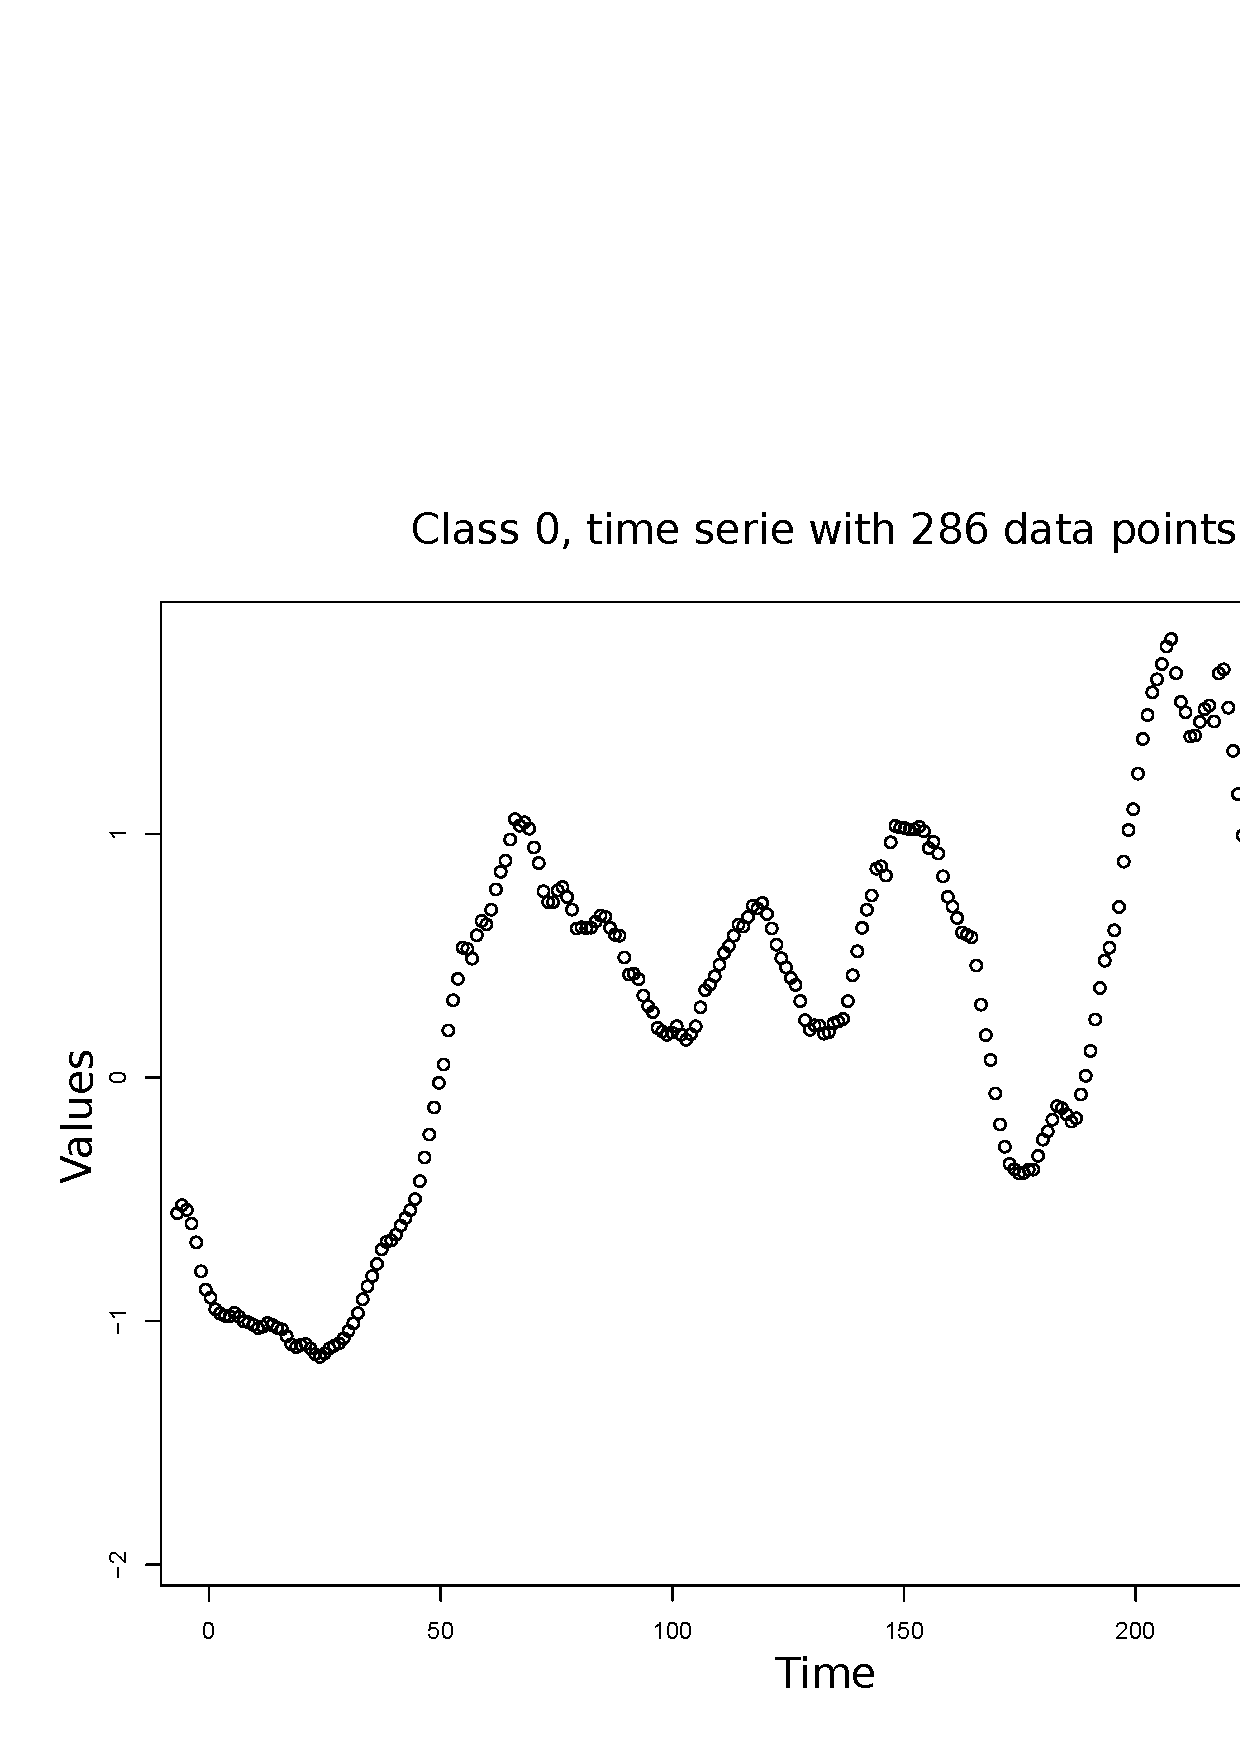
\includegraphics[scale=0.23]{coffee_0_ts}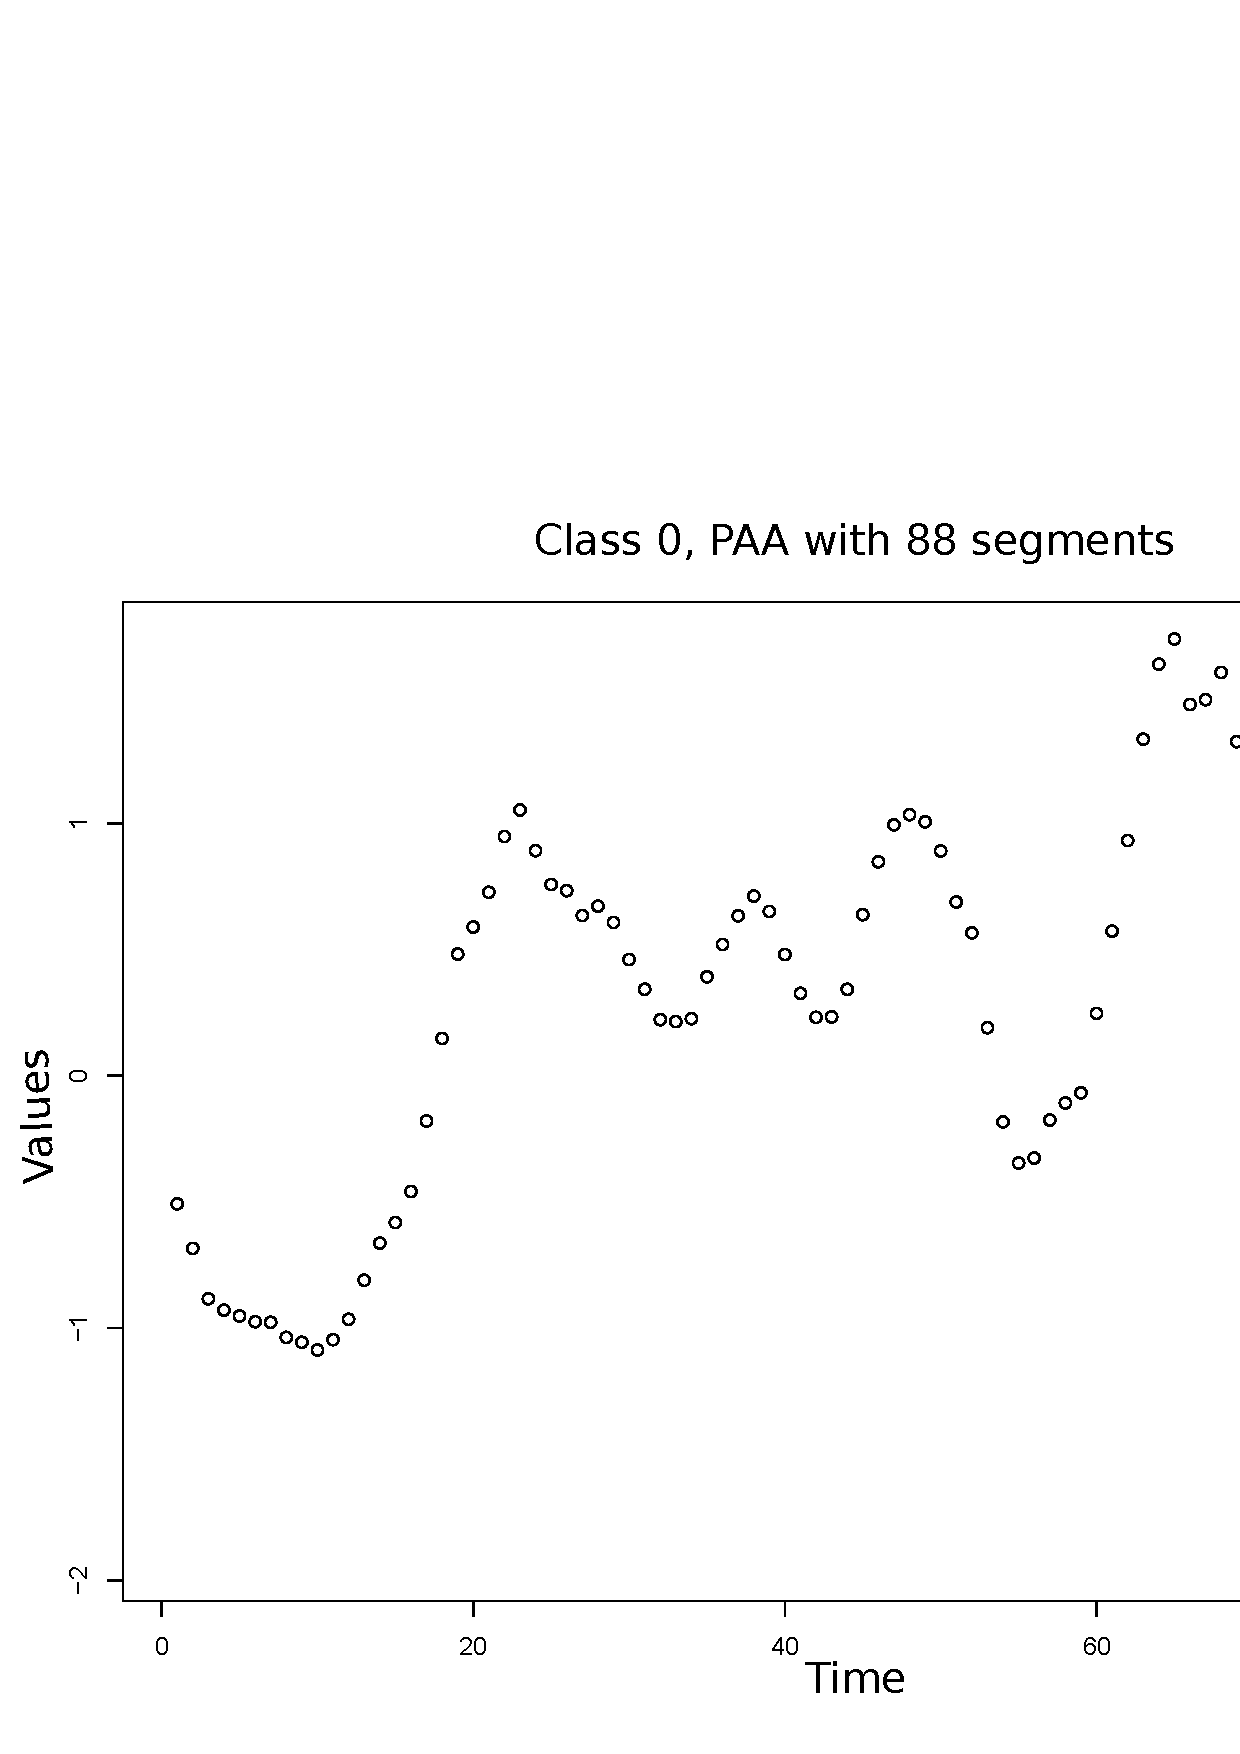
\includegraphics[scale=0.23]{coffee_0_paa_88}

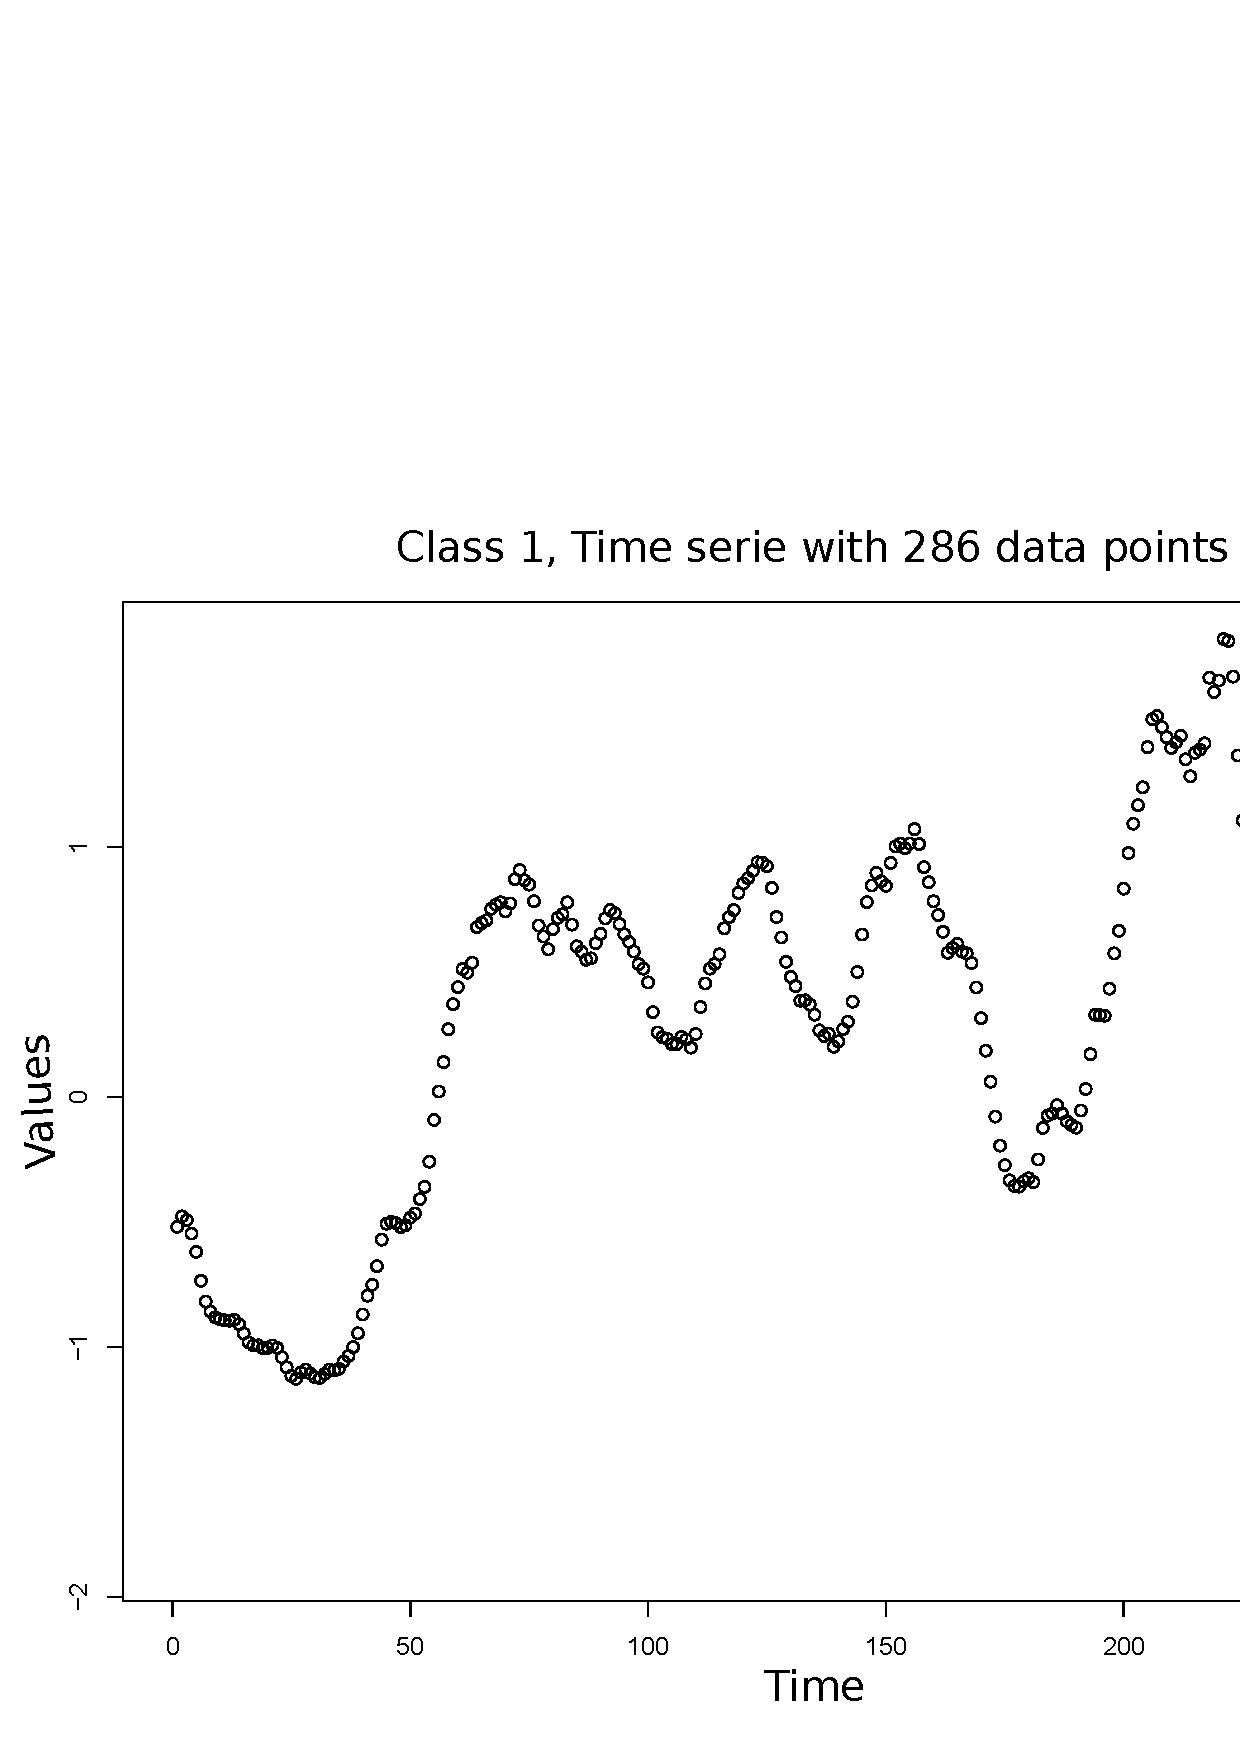
\includegraphics[scale=0.23]{coffee_1_ts}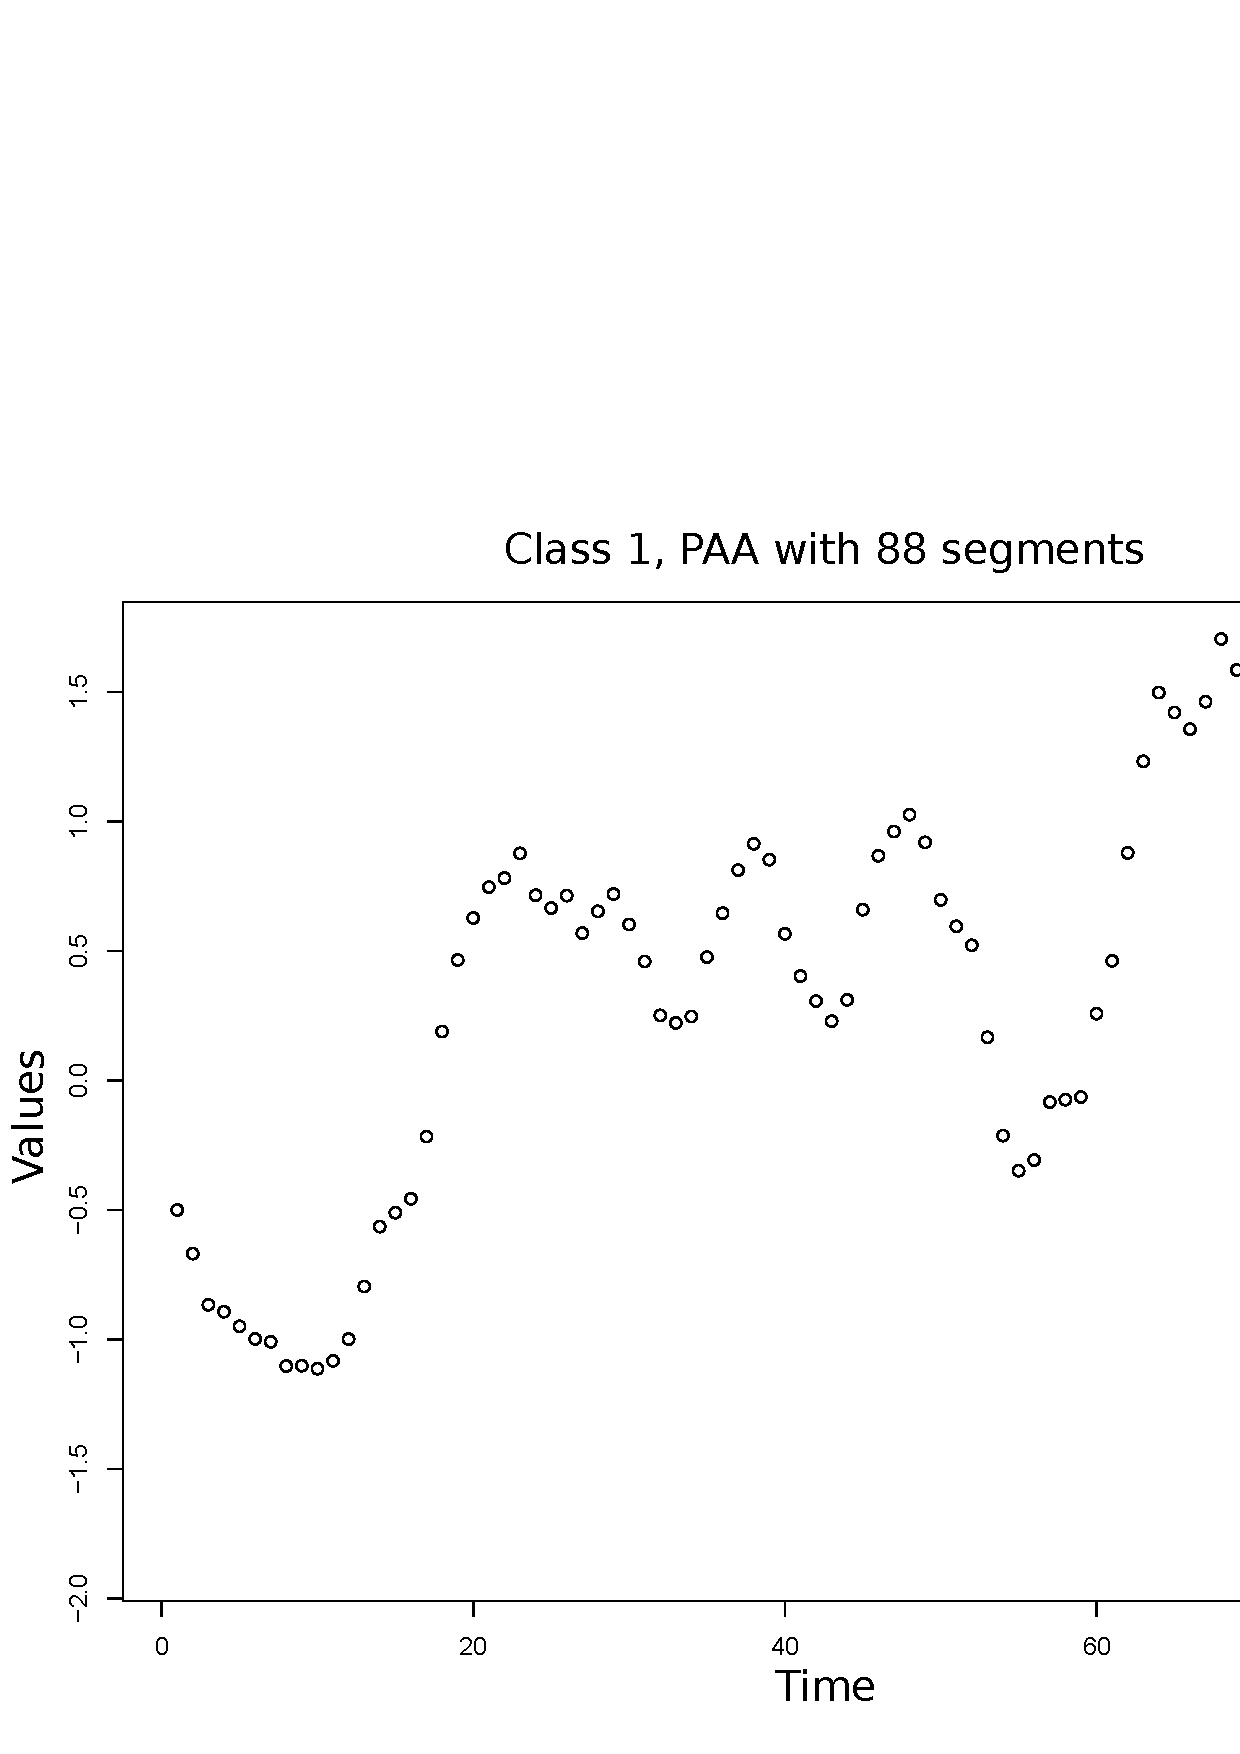
\includegraphics[scale=0.23]{coffee_1_paa_88}

\caption{Visual comparison of two time series from the two classes of the coffee dataset. Left: the original time series (286 data points), right:  representation using PAA with 88 segments}

\label{coffee}
\end{figure}


\subsubsection{Classification}

PAA is used by ShapeDTW \cite{zhao2016shapedtw} and DTW\_F \cite{Kate2016} to classify time series. However, to evaluate the actual impact of the segment number considered on the classification, we tested FDTW to choose the
number of segments to use with 1NN and PDTW. 


PDTW was designed to speed up the calculation of DTW without degrading the accuracy. In our experiments, we observe that when the number of segments is chosen, this may even lead to an improvement of the results of the classification.




 \paragraph{}\textbf{Quality of the number of segments:}   \\
 A segment number $N_1$ is better than a segment number $N_2$ if the classification
 error associated with $N_1$ is smaller than that associated with $N_2$. So, to evaluate the
 quality of our heuristic FDTW, we compared its classification errors with that of IDDTW.
  The classification error  was computed from the results of the 3 fold cross validation 
  applied on the training set. IDDTW tested all the values of $N$ that were equal to a power of two and kept the one that had  a minimum
classification error (Table \ref{error_trainingset}).



 \paragraph{}\textbf{Application:}  \\
According to the announcement in \textbf{Lemma 1}, the classification error of FDTW during the learning phase (training error) is less
than or equal to that of DTW for all the considered datasets.  We used \textbf{Wilcoxon signed rank test} with continuity
correction to test the significance of FDTW against IDDTW.  The Wilcoxon signed rank test gives a
p-values, \textbf{ p $<$ 0.01}, which demonstrates that FDTW achieves a
significant reduction of the classification error of IDDTW. This also demonstrates that FDTW allows
to find segment numbers for PAA that are of better quality than those found by IDDTW during the learning phase.

\begin{center}
\tablefirsthead{%
\hline 
$N^{\circ}$ & \textbf{Datasets}  & \textbf{DTW} & \textbf{IDDTW} & \textbf{N} &
\textbf{FDTW} & \textbf{N} \tabularnewline 

 & \textbf{(training set)}&           &   &  &  &  \tabularnewline \hline} 
\tablehead{%
\hline 
$N^{\circ}$ & \textbf{Datasets}  & \textbf{DTW} & \textbf{IDDTW} & \textbf{N} &
\textbf{FDTW} & \textbf{N} \tabularnewline 

 & \textbf{(training set)}&           &   &  &  &  \tabularnewline \hline}

\tabletail{%
\hline
\multicolumn{7}{|r|}{\small\sl continued on next page}\\
\hline}
\tablelasttail{\hline}

\bottomcaption{Classification errors associated with the number of segments \textbf{N} chosen by the
heuristics IDDTW and FDTW. When two numbers of segments $N_1$ and $N_2$ are associated with the same
classification error, the smallest is considered. The classification error  is calculated based on the 3 fold cross validation   applied on the training set.}

\label{error_trainingset}
\small
\begin{supertabular}{c|ll|ll|ll}
1 & 50Words & 0.349 & 0.340 & 256 & 0.318 & 80\tabularnewline
2 & Adiac & 0.462 & 0.426 & 128 & 0.426 & 140\tabularnewline
3 & ArrowHead & 0.250 & 0.167 & 16 & 0.111 & 14\tabularnewline
4 & Beef & 0.567 & 0.900 & 8 & 0.567 & 169\tabularnewline
5 & Car & 0.400 & 0.233 & 8 & 0.217 & 385\tabularnewline
6 & CBF & 0.000 & 0.000 & 128 & 0.000 & 22\tabularnewline
7 & Coffee & 0.033 & 0.133 & 64 & 0.000 & 88\tabularnewline
8 & Cricket\_X & 0.210 & 0.244 & 256 & 0.190 & 84\tabularnewline
9 & Cricket\_Y & 0.279 & 0.285 & 256 & 0.272 & 214\tabularnewline
10 & Cricket\_Z & 0.267 & 0.272 & 256 & 0.249 & 250\tabularnewline
11 & DistalPhalanxOutlineAgeGroup & 0.570 & 0.541 & 16 & 0.534 & 14\tabularnewline
12 & DistalPhalanxTW & 0.375 & 0.339 & 16 & 0.317 & 40\tabularnewline
13 & Earthquakes & 0.266 & 0.266 & 512 & 0.223 & 101\tabularnewline
14 & ECG & 0.240 & 0.170 & 8 & 0.170 & 11\tabularnewline
15 & ECGFive Days & 0.387 & 0.220 & 32 & 0.220 & 7\tabularnewline
16 & Face (all) & 0.875 & 0.873 & 128 & 0.870 & 50\tabularnewline
17 & Face (four) & 0.208 & 0.125 & 32 & 0.083 & 140\tabularnewline
18 & Fish & 0.343 & 0.314 & 16 & 0.303 & 27\tabularnewline
19 & Gun-point & 0.201 & 0.039 & 32 & 0.020 & 38\tabularnewline
20 & Ham & 0.650 & 0.512 & 32 & 0.512 & 32\tabularnewline
21 & Haptics & 0.587 & 0.536 & 64 & 0.516 & 239\tabularnewline
22 & InlineSkate & 0.519 & 0.519 & 64 & 0.499 & 48\tabularnewline
23 & ItalyPower Demand & 0.045 & 0.060 & 8 & 0.045 & 20\tabularnewline
24 & Lightning-2 & 0.183 & 0.150 & 16 & 0.100 & 179\tabularnewline
25 & Lightning-7 & 0.315 & 0.344 & 64 & 0.200 & 155\tabularnewline
26 & Medical Images & 0.286 & 0.307 & 64 & 0.278 & 94\tabularnewline
27 & MiddlePhalanxTW & 0.429 & 0.442 & 32 & 0.429 & 80\tabularnewline
28 & MoteStrain & 0.246 & 0.246 & 16 & 0.190 & 46\tabularnewline
29 & OliveOil & 0.367 & 0.367 & 32 & 0.333 & 423\tabularnewline
30 & OSU leaf & 0.310 & 0.335 & 32 & 0.270 & 33\tabularnewline
31 & Plane & 0.000 & 0.000 & 32 & 0.000 & 32\tabularnewline
32 & ProximalPhalanxTW & 0.317 & 0.283 & 4 & 0.283 & 4\tabularnewline
33 & ShapeletSim & 0.786 & 0.246 & 8 & 0.143 & 45\tabularnewline
34 & SonyAIBORobot Surface & 0.198 & 0.095 & 16 & 0.048 & 22\tabularnewline
35 & SonyAIBORobot Surface II & 0.148 & 0.111 & 64 & 0.037 & 42\tabularnewline
36 & Swedish & 0.250 & 0.238 & 64 & 0.218 & 59\tabularnewline
37 & Symbols & 0.037 & 0.037 & 32 & 0.000 & 34\tabularnewline
38 & Synthetic Control & 0.350 & 0.410 & 32 & 0.350 & 60\tabularnewline
39 & Trace & 0.000 & 0.000 & 64 & 0.000 & 108\tabularnewline
40 & Two patterns & 0.000 & 0.000 & 32 & 0.000 & 32\tabularnewline
41 & TwoLead ECG & 0.125 & 0.083 & 64 & 0.083 & 52\tabularnewline
42 & Wafer & 0.014 & 0.012 & 8 & 0.008 & 111\tabularnewline
43 & Wine & 0.684 & 0.632 & 128 & 0.632 & 20\tabularnewline
44 & Words Synonyms & 0.419 & 0.423 & 64 & 0.382 & 57\tabularnewline
45 & Yoga & 0.233 & 0.187 & 128 & 0.187 & 356\tabularnewline
\hline 
\end{supertabular}
\end{center}
 
 

 \paragraph{}\textbf{Comparison with IDDTW:}  \\
To evaluate the quality of FDTW, we compared its classification errors with
that of IDDTW  and the minimal one. The minimal classification error was find by applying Brute-force search (BF) on both training set and testing set. FDTW and IDDTW used
the training set to find the segment number $N$ with minimal training error using 3 fold cross validation, and then used this number of segments on the testing set to compute the classification error. The value of the segment number $N$ found on the training set may in some cases not be appropriate for the testing set. It is a  generalization error, which is due to the representativeness of the training set (Table \ref{error}).  
 
If two numbers of
segments $N_1$ and $N_2$ are associated with the same training error, we retain the largest.
IDDTW tested all the values of $N$ that were equal to a power of two during the learning phase and kept the one that had  a minimum classification error.  





\begin{center}
\tablefirsthead{%
\hline 

\multicolumn{4}{|c|}{\textbf{\cite{UCRArchive}}} & \multicolumn{6}{c|}{\textbf{Our experiments}}\tabularnewline
\hline 
$N^{\circ}$  & \textbf{1NN } & \textbf{1NN } & \textbf{1-NN }  & \textbf{Brute} & \textbf{N(}$\ell$\textbf{)} & \textbf{IDDTW} & \textbf{N(}$\ell$\textbf{)} & \textbf{FDTW} & \textbf{N(}$\ell$\textbf{)}\tabularnewline
 & \textbf{Eucli } & \textbf{DTW} & \textbf{DTW (r)}  & \textbf{force } &  &  &  &  & \tabularnewline
 & \textbf{dean} &  &   & \textbf{search} &  &  &  &  & \tabularnewline
 & \textbf{distance} &  &  &  &  &  &  &  &  \tabularnewline
\hline }
\tablehead{%
\hline
\multicolumn{10}{|l|}{\small\sl continued from previous page}\\
\hline 

\multicolumn{4}{|c|}{\textbf{\cite{UCRArchive}}} &
\multicolumn{6}{c|}{\textbf{Our experiments}}\tabularnewline
\hline 
$N^{\circ}$  & \textbf{1NN } & \textbf{1NN } & \textbf{1-NN }  & \textbf{Brute} & \textbf{N(}$\ell$\textbf{)} & \textbf{IDDTW} & \textbf{N(}$\ell$\textbf{)} & \textbf{FDTW} & \textbf{N(}$\ell$\textbf{)}\tabularnewline
 & \textbf{Eucli } & \textbf{DTW} & \textbf{DTW (r)}  & \textbf{force } &  &  &  &  & \tabularnewline
 & \textbf{dean} &  &   & \textbf{search} &  &  &  &  & \tabularnewline
 & \textbf{distance} &  &  &  &  &  &  &  &  \tabularnewline
\hline }
\tabletail{%
\hline
\multicolumn{10}{|r|}{\small\sl continued on next page}\\
\hline}
\tablelasttail{\hline}


\bottomcaption{Comparison of generalization errors. In \textbf{italics}, the smallest generalization
error. In \textbf{bold}, the smallest generalization error between IDDTW and FDTW. \textbf{N }is the number of segments selected
and $\ell$ is the number of data points in a segment $(l = \lfloor\frac{n}{N}\rfloor)$. The generalization error  is computed on the testing set. Note : DTW (r) is a constraint version of DTW where the number of consecutive data points that can be compared to a single point during the warping is bounded.  r represents the size of the warping windows}

\label{error}
\small
\begin{supertabular}{|p{0.15cm}|p{1cm}ll|ll|ll|ll|}
1 & 0.369 & 0.310 & 0.242 (6)  & 0.262 & 251(1) & \textbf{0.268} & 256(1) &
\textbf{0.268} & 258(1)\tabularnewline 


2 & 0.389 & 0.396 & 0.391 (3)  & 0.379 & 162(1) & 0.432 & 128(1) & \textbf{0.414}
& 143(1)\tabularnewline 


3 & 0.333 & 0.367 & 0.333 (0)  & 0.233 & 286(2) & \textbf{0.3} & 8(59) & 0.367 &
94(5)\tabularnewline 




4 & 0.425 & 0.274 & 0.288 (5)  & \emph{0.192} & 150(2) & \textbf{0.301} & 64(5) &
\textbf{0.301} & 170(2)\tabularnewline 




5 & 0.26 & 0.25 & 0.253 (5)  & 0.233 & 27(2) &  \textbf{0.283}  & 2(40) &
\textbf{0.283} & 385(2)\tabularnewline 







6 & 0.148 & 0.003 & 0.004 (11)  & \emph{0} & 118(1) & 0.003 & 128(1) &
\textbf{\emph{0.001}} & 128(1)\tabularnewline 


7 & 0.000 & 0.000 & 0.000 (0)  & \emph{0} & 13(22) & \textbf{\emph{0}} & 64(4) &
\textbf{\emph{0.000}} & 286(1)\tabularnewline 


8 & 0.423 & 0.246 & 0.228 (10)  & 0.228 & 142(2) & \textbf{0.256} & 256(1) &
0.269 & 84(4)\tabularnewline 


9 & 0.433 & 0.256 & 0.238 (17)  & 0.231 & 271(1) & \textbf{0.241} & 256(1) &
0.244 & 294(1)\tabularnewline 


10 & 0.413 & 0.246 & 0.254 (5)  & 0.221 & 249(1) & \textbf{0.223} & 256(1) & 0.233
& 276(1)\tabularnewline 


11 & 0.218 & 0.208 & 0.228 (1)  & 0.2 & 78(1) &  0.225  & 16(5) & \textbf{0.223} &
80(1)\tabularnewline 


12 & 0.273 & 0.29 & 0.272 (0)  & \emph{0.263} & 35(2) &  0.288  & 16(5) &
\textbf{0.278} & 80(1)\tabularnewline 


13 & 0.326 & 0.258 & 0.258 (22)  &\emph{0.198} & 176(2) & \textbf{ 0.258}  & 512(1) &
0.276 & 101(5)\tabularnewline 


14 & 0.120 & 0.230 & 0.120 (0)  & 0.13 & 38(3) & 0.19 & 8(12) & \textbf{0.180} &
11(9)\tabularnewline 


15 & 0.203 & 0.232 & 0.203 (0)  & 0.117 & 11(12) & 0.289 & 32(4) & \textbf{0.117}
& 11(12)\tabularnewline 


16 & 0.286 & 0.192 & 0.192 (3)  & 0.091 & 79(2) & 0.194 & 128(1) & \textbf{0.148}
& 99(1)\tabularnewline 


17 & 0.216 & 0.170 & 0.114 (2)  & 0.08 & 107(3) & 0.352 & 32(11) & \textbf{0.102}
& 140(3)\tabularnewline 


18 & 0.217 & 0.177 & 0.154(4)  & 0.154 & 149(3) & 0.257 & 16(29) & \textbf{0.177} &
27(17)\tabularnewline 


19 & 0.087 & 0.093 & 0.087 (0)  & 0.02 & 38(4) & 0.073 & 32(5) & \textbf{0.020} &
38(4)\tabularnewline 


20 & 0.4 & 0.533 & 0.400 (0)  & 0.343 & 21(20) & \textbf{ 0.026}  & 32(13) & 0.432
& 32(13)\tabularnewline 


21 & 0.630 & 0.623 & 0.588 (2)  & 0.549 & 328(3) & \textbf{0.588} & 64(17) &
0.594 & 948(1)\tabularnewline 


22 & 0.658 & 0.616 & 0.613 (14)  & 0.578 & 1770(1) & 0.627 & 64(29) &
\textbf{0.622} & 171(11)\tabularnewline 


23 & 0.045 & 0.050 & 0.045 (0)  & 0.033 & 20(1) & 0.043 & 8(3) & \textbf{0.033} &
24(1)\tabularnewline 


24 & 0.133 & 0.167 & 0.133 (0)  & 0.1 & 191(3) & 0.167 & 32(18) & \textbf{0.100}
& 234(2)\tabularnewline 


25 & 0.267 & 0.267 & 0.233 (1)  & 0.183 & 52(11) &  \textbf{0.367 } & 8(72) &
\textbf{0.367} & 377(1)\tabularnewline 


26 & 0.038 & 0 & 0.000 (6)  & \emph{0} & 35(4) & \textbf{ }\textbf{\emph{0}}\textbf{ }
& 128(1) & \textbf{\emph{0}} & 135(1)\tabularnewline 


27 & 0.439 & 0.416 & 0.419 (2)  & \emph{0.398} & 27(2) & \textbf{ 0.414 } & 32(2) &
0.416 & 80(1)\tabularnewline 


28 & 0.121 & 0.165 & 0.134 (1)  & 0.135 & 14(6) & 0.197 & 16(5) & \textbf{0.165} &
84(31)\tabularnewline 


29 & 0.246 & 0.131 & 0.131 (6)  &  \emph{0.082} & 70(9) & 0.246 & 16(40) &
\textbf{0.180} & 524(1)\tabularnewline 


30 & 0.479 & 0.409 & 0.388 (7)  & 0.364 & 31(14) & \textbf{0.372} & 32(13) &
0.409 & 35(12)\tabularnewline 


31 & 0.316 & 0.263 & 0.253 (20)  & 0.255 & 95(1) & \textbf{0.271} & 64(2) & 0.280
& 34(3)\tabularnewline 


32 & 0.292 & 0.263 & 0.263 (6)  & 0.24 & 75(1) &  \textbf{0.288 } & 4(20) &
\textbf{0.288} & 4(20)\tabularnewline 


33 & 0.461 & 0.35 & 0.300 (3)  & 0.083 & 54(9) &  0.239  & 64(7) & \textbf{0.122} &
48(10)\tabularnewline 


34 & 0.305 & 0.275 & 0.305 (0)  & 0.206 & 37(2) & \textbf{0.208} & 16(4) & 0.304 &
26(3)\tabularnewline 


35 & 0.141 & 0.169 & 0.141 (0)  & 0.14 & 5(13) & 0.197 & 16(4) & \textbf{0.178} &
45(1)\tabularnewline 


36 & 0.211 & 0.208 & 0.154 (2)  & 0.165 & 59(2) & \textbf{0.195} & 64(2) & 0.208
& 55(2)\tabularnewline 


37 & 0.100 & 0.050 & 0.062 (8)  & 0.044 & 376(1) & \textbf{0.059} &
32(12) & 0.060 & 34(12)\tabularnewline 


38 & 0.120 & 0.007 & 0.017 (6)  & 0.007 & 60(1) & 0.437 & 2(30) & \textbf{0.007}
& 60(1)\tabularnewline 


39 & 0.240 & 0.000 & 0.010 (3)  & \emph{0} & 47(6) & \textbf{\emph{0}} &
64(4) & \textbf{\emph{0}} & 275(1)\tabularnewline 


40 & 0.090 & 0.000 & 0.002 (4)  & \emph{0} & 21(6) & \textbf{\emph{0}} &
64(2) & \textbf{\emph{0}} & 128(1)\tabularnewline 


41 & 0.253 & 0.096 & 0.132 (5)  & 0.045 & 55(1) & 0.073 & 32(3) & 0.112 &
70(1)\tabularnewline 


42 & 0.005 & 0.020 & 0.005 (1)  & 0.007 & 109(1) & 0.013 & 8(19) & \textbf{0.008} &
95(2)\tabularnewline 


43 & 0.389 & 0.426 & 0.389 (0)  & 0.204 & 3(78) &  0.463  & 20(11) &
\textbf{0.37} & 128(1)\tabularnewline 


44 & 0.382 & 0.351 & 0.252 (8)  & 0.337 & 133(2) & 0.365 & 64(4) & \textbf{0.343} &
135(2)\tabularnewline 


45 & 0.170 & 0.164 & 0.155 (2)  & 0.149 & 117(4) & 0.158 & 128(3) &
\textbf{0.154} & 384(1)\tabularnewline


\hline 
$\overline{X}$  & 0.268 & 0.227 & 0.242 &  0.175 &  & 0.232 &  & 0.214 & \tabularnewline


\hline 
\end{supertabular}
\end{center}



The results of our experiments showed that FDTW is more performant than IDDTW. Actually, FDTW resulted in a
lower generalization error than IDDTW on 22 datasets and the same generalization error than IDDTW on 8
datasets.  The Wilcoxon signed rank test gives a
p-values, \textbf{ 0.01 $<$ p $\leq$ 0.05}, which demonstrates that FDTW achieved a
significant reduction of the generalization error of IDDTW. Results also showed that FDTW was able to
find the minimum error for 9 datasets (Coffee, ECGFiveDays, Gun-point, ItalyPowerDemand, OliveOil, Plane, Synthetic control, Trace, Two
patterns) and outperforms the smallest classification error reported in the literature on
dataset CBF ($N^{\circ} 5$).




\paragraph{}\textbf{Heuristic execution speed\footnote{Note: The experiments were conducted on a PC with an Intel Core i7 processor, 16GB of RAM and a Windows 7 64-bit operating system.}: }\\
As already suggested by the time complexity of both FDTW and IDDTW heuristics, IDDTW
tests fewer candidates than FDTW and is therefore faster. However, the number of candidates tested
by FDTW reduces exponentially with the length of the time series (Figure
\ref{NumberOfValuesTested}).
Actually, the number of candidates to be tested ranges from 1 to $n$, $n$ being the  length of time
series, and FDTW considers $\sqrt{n}$ candidates for each iteration.



\begin{figure}
\center
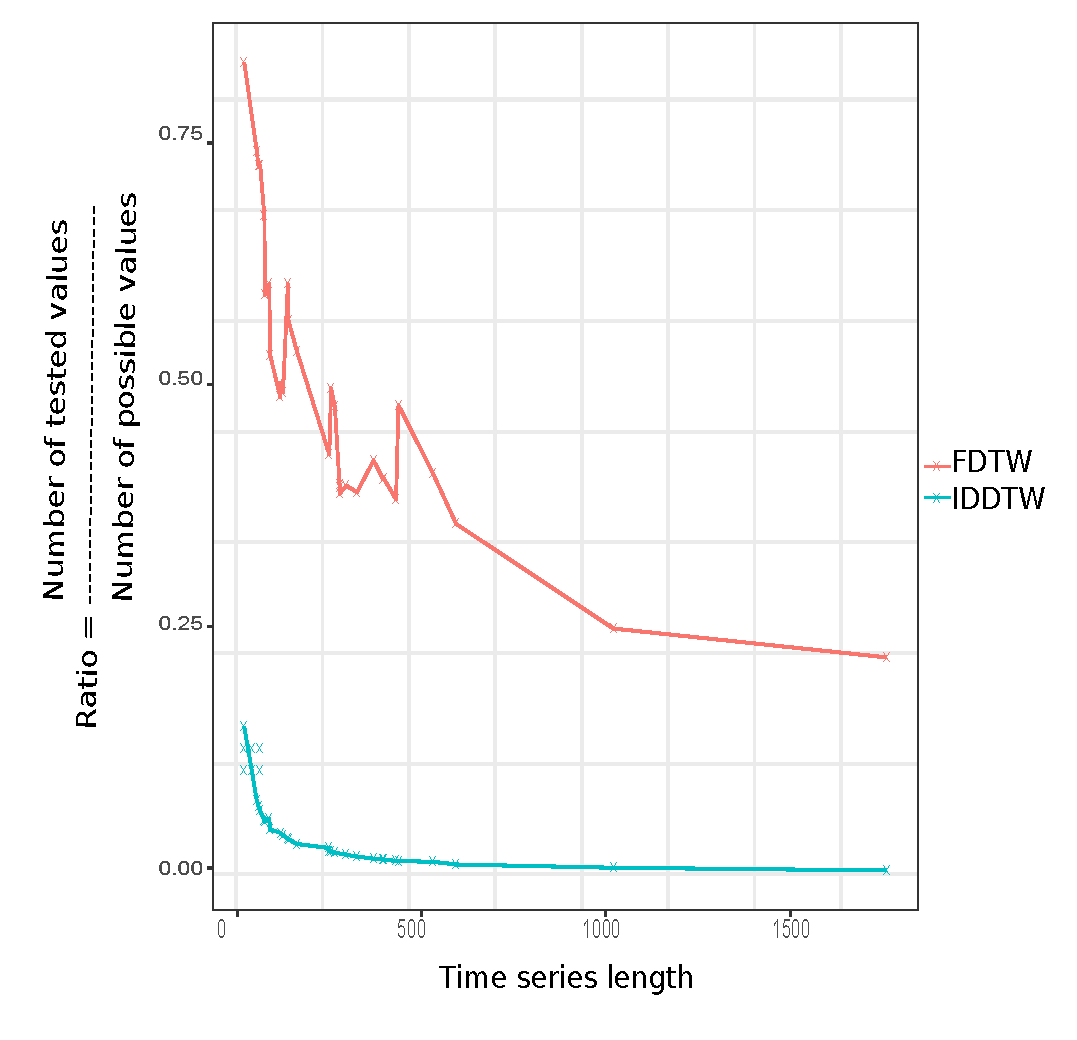
\includegraphics[width=23pc,height=19pc]{nombre_de_candidats_testees}
\caption{Comparison of the number of tested values of the parameter number of segments with
the FDTW and IDDTW.  Datasets are sorted according to
the length of the time series (x-axis). }

\label{NumberOfValuesTested}

\end{figure}

In average, FDTW is 8 times faster than Brute-force search with an average execution time of 176 minutes
against 1386 minutes for Brute-force search. IDDTW is 7 times faster than FDTW and remains
the fastest with an average execution time of 24 minutes. The execution time increases with the length of the time series (Figure 
\ref{tempsDeCalcul}). The increase of Brute-force search execution time is much more important than that of FDTW
and IDDTW, particularly on datasets that contain more than 600 points (e.g. Lightning-2). 

\begin{figure}
\center
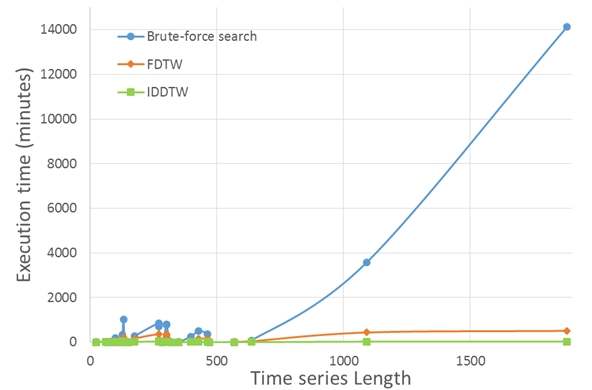
\includegraphics[width=22pc,height=15pc]{tempsDeCalcul2.jpg}
\caption{Comparison of the execution time of
the Brute-force search algorithm, FDTW and IDDTW. }

\label{tempsDeCalcul}

\end{figure}




 \paragraph{}\textbf{Comparison with other classification algorithms:}  \\
To evaluate the quality of FDTW, we compared its classification errors (generalization error) with that of 35 other classification algorithms \cite{bagnall2016great} of the literature on 84 datasets of UCR archive{{}}.
 The performances of the algorithms are compared using 
the Nemenyi test that compares all the algorithms pairwise and  provides an intuitive way to
visualize the results (Fig. \ref{cd2}). The Nemenyi test allows ranking  classification algorithms according to their average accuracy on 84 datasets.
 FDTW obtained good results on the simulated datasets in terms of average accuracy (3rd / 37 algorithms) because  data of the training set and of the testing set are generated by the same models.

\begin{figure}
\centering
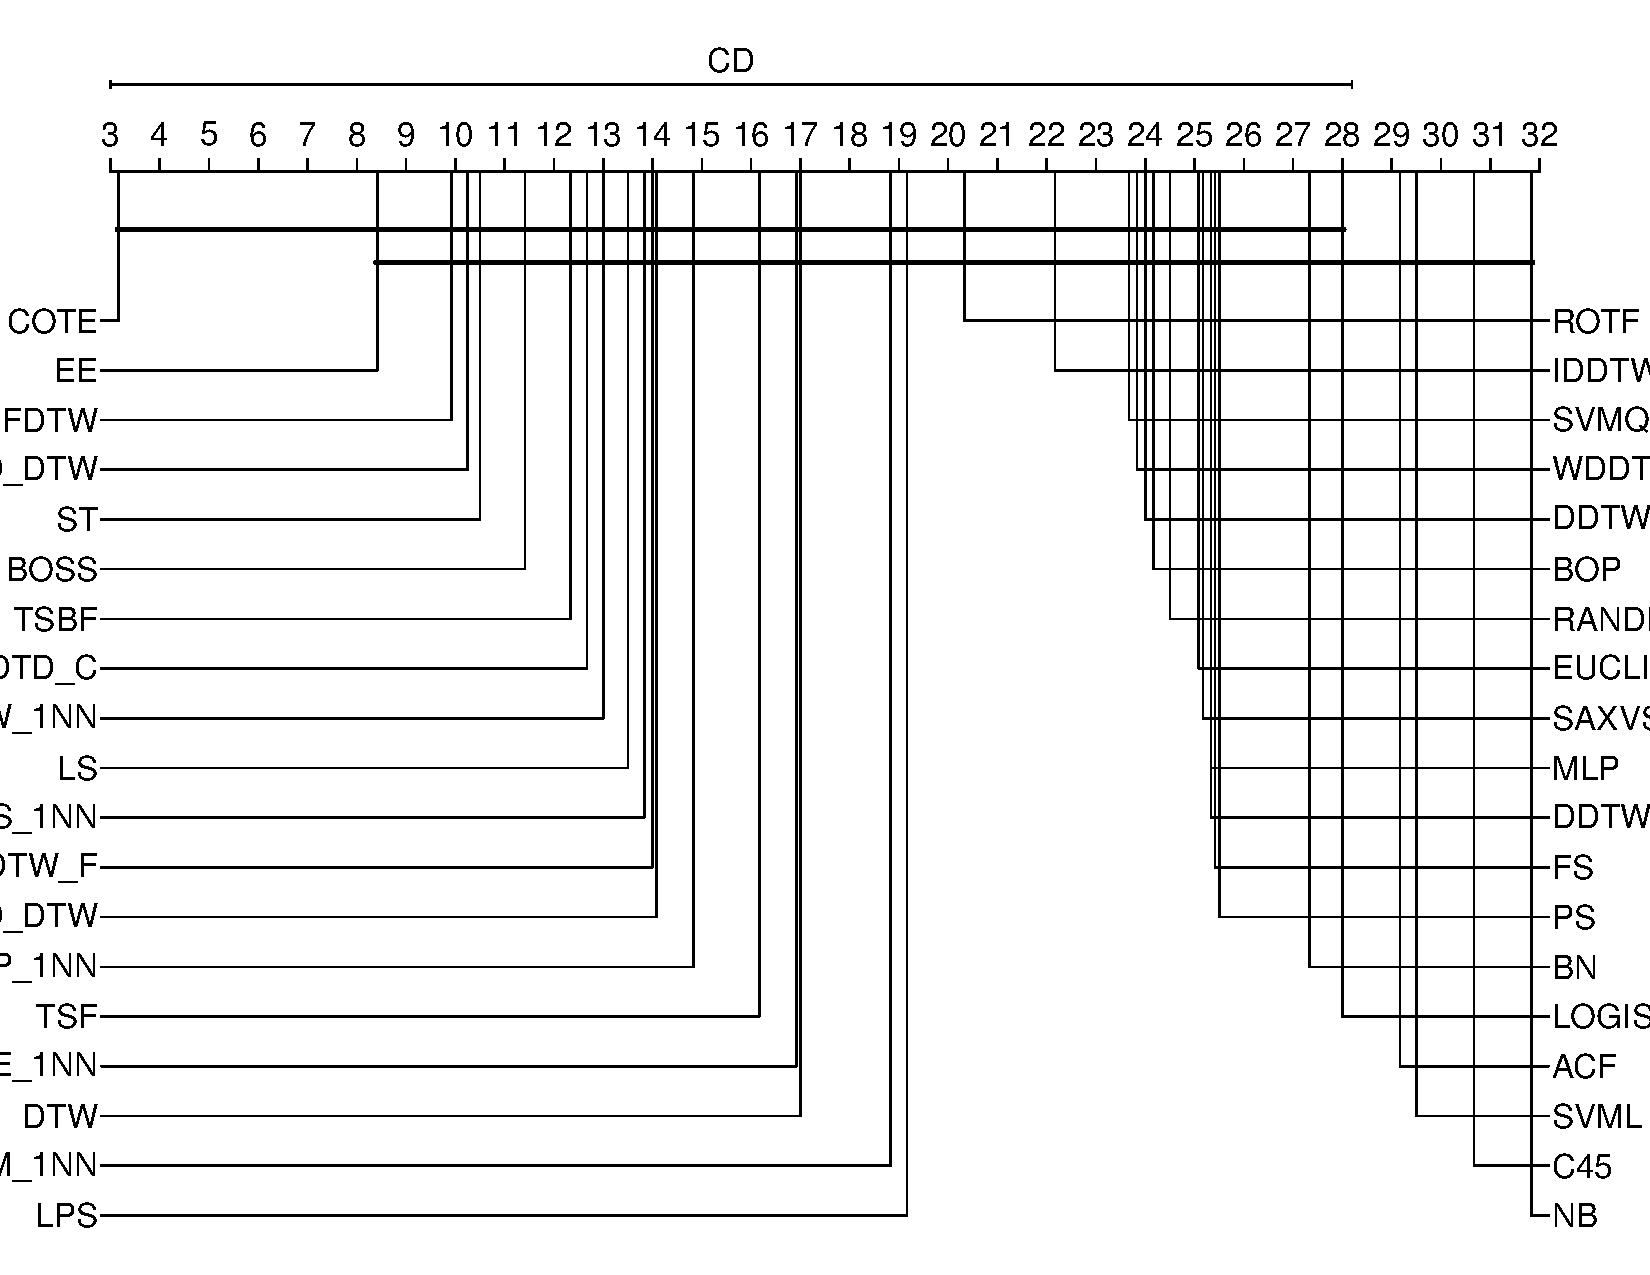
\includegraphics[scale=0.33]{images/cd1}
\caption{Critical difference diagram for FDTW and $36$ other classification algorithms on 6 simulated datasets. FDTW is ranked 3rd / 37 algorithms}

\label{cd2}
\end{figure}



However, to evaluate the significance of the difference between the 35 classification algorithms on 84 datasets, we used the Wilcoxon signed rank test with continuity correction, which has a higher statistical power than Nemenyi test. The results of these tests  show that despite data compression, 
\begin{itemize}
  \item  FDTW had a better performance than Naive Bayes (NB), C45,  logistic regression (Logistic), BN;
  \item FDTW had a similar performance as 26 other algorithms in the literature, namely: SVMQ, RANDF, ROTF, MLP, EUCLIDEAN\_1\_NN, DDTW\_R1\_1NN, DDTW\_RN\_1NN, ERP\_1NN, LCSS\_1NN, MSM\_1NN, TWE\_1NN, WDDTW\_1NN, WDTW\_1NN, DD\_DTW, DTD\_C, LS, BOP, SAXVSM, TSF, TSBF, LPS, PS, CID\_DTW, SVML, FS, ACF;
  \item Only five algorithms DTW\_F, Shapelet Transform (ST), BOSS, Elastic Ensemble (EE) and COTE performed better overall than FDTW.
\end{itemize}

These results demonstrate the competitiveness of FDTW. Moreover, this algorithm
outperforms the best result reported in the literature on  UWaveGestureLibraryAll dataset (Fig.
\ref{geste}).
The challenge with this dataset is to recognize the gesture made by a user
from measurements made by accelerometers. As reported in \cite{Bagnall} the best accuracy obtained
on this dataset is 83.44\% with TSBF algorithm; FDTW outperforms this result and allows to obtain \textbf{91.87\%} of accuracy.


\begin{figure}
\center
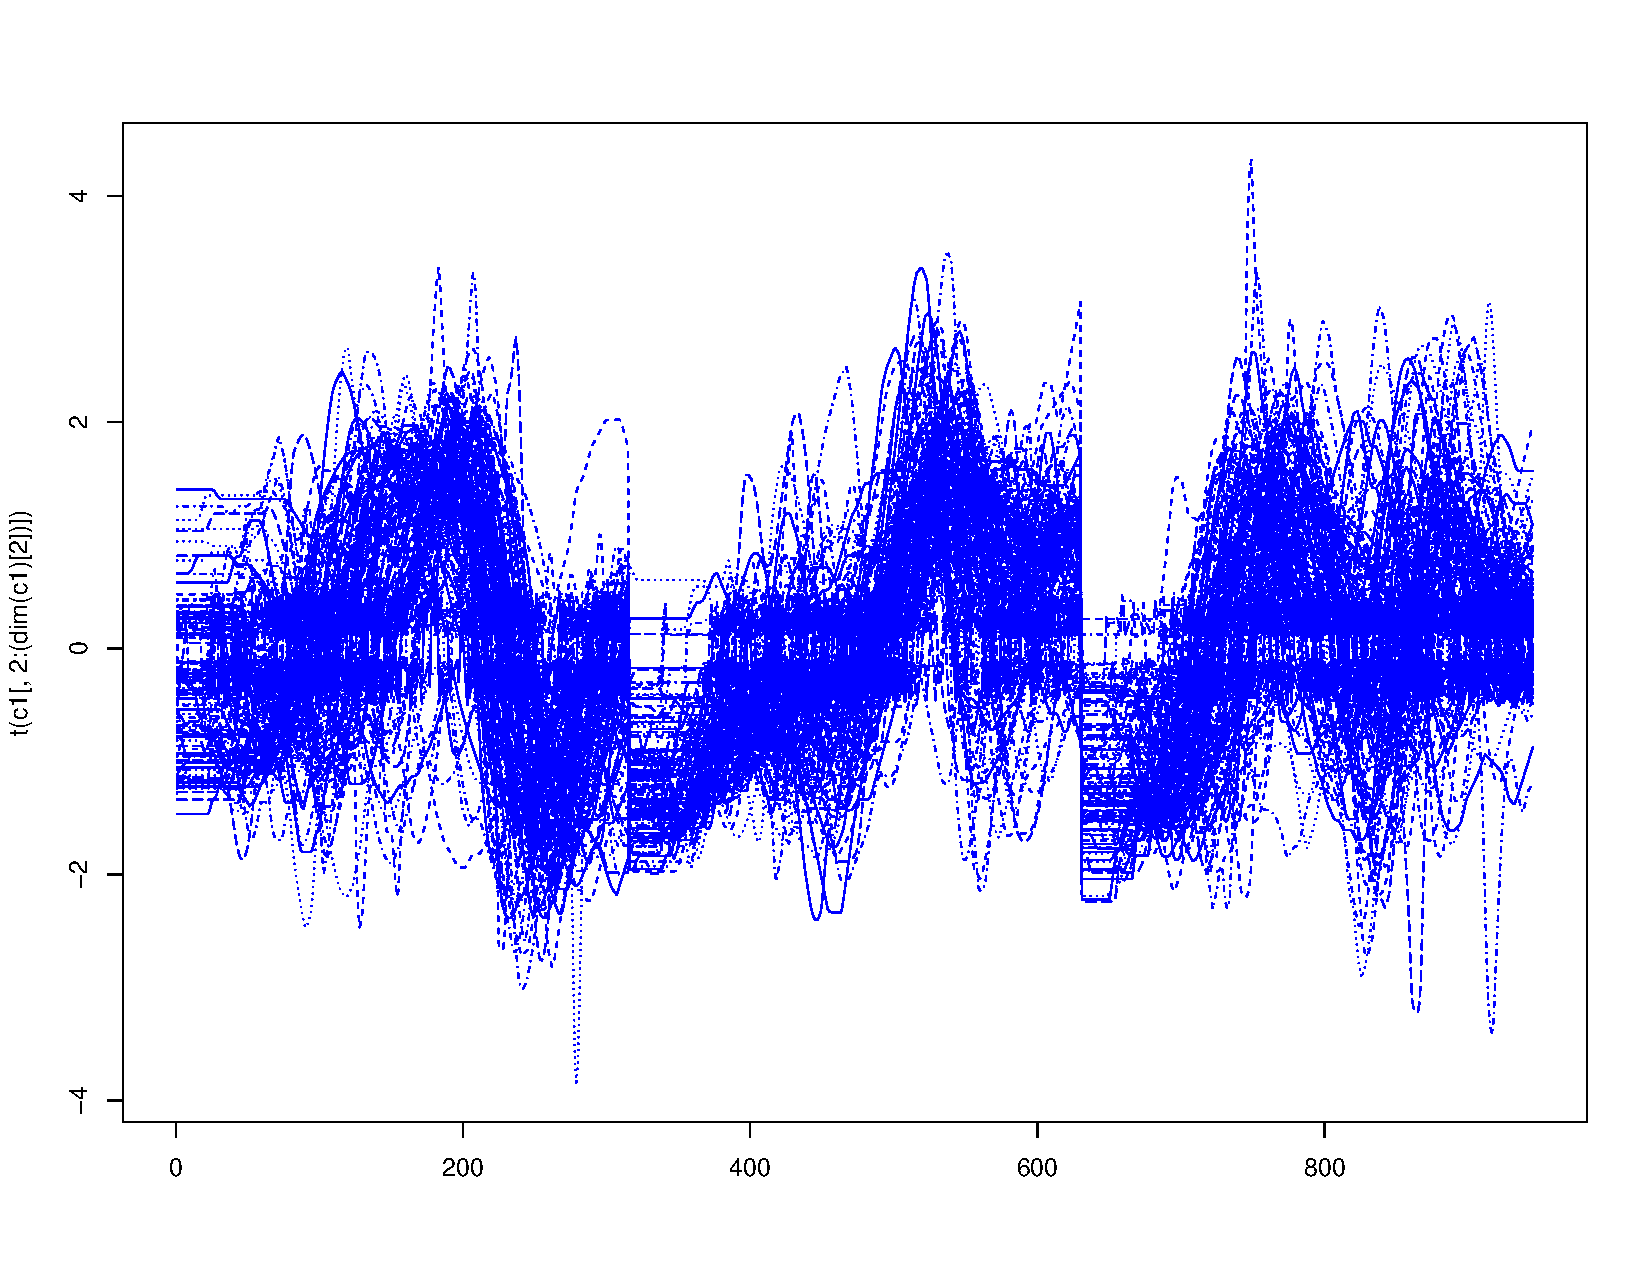
\includegraphics[scale=0.1]{images/c1}
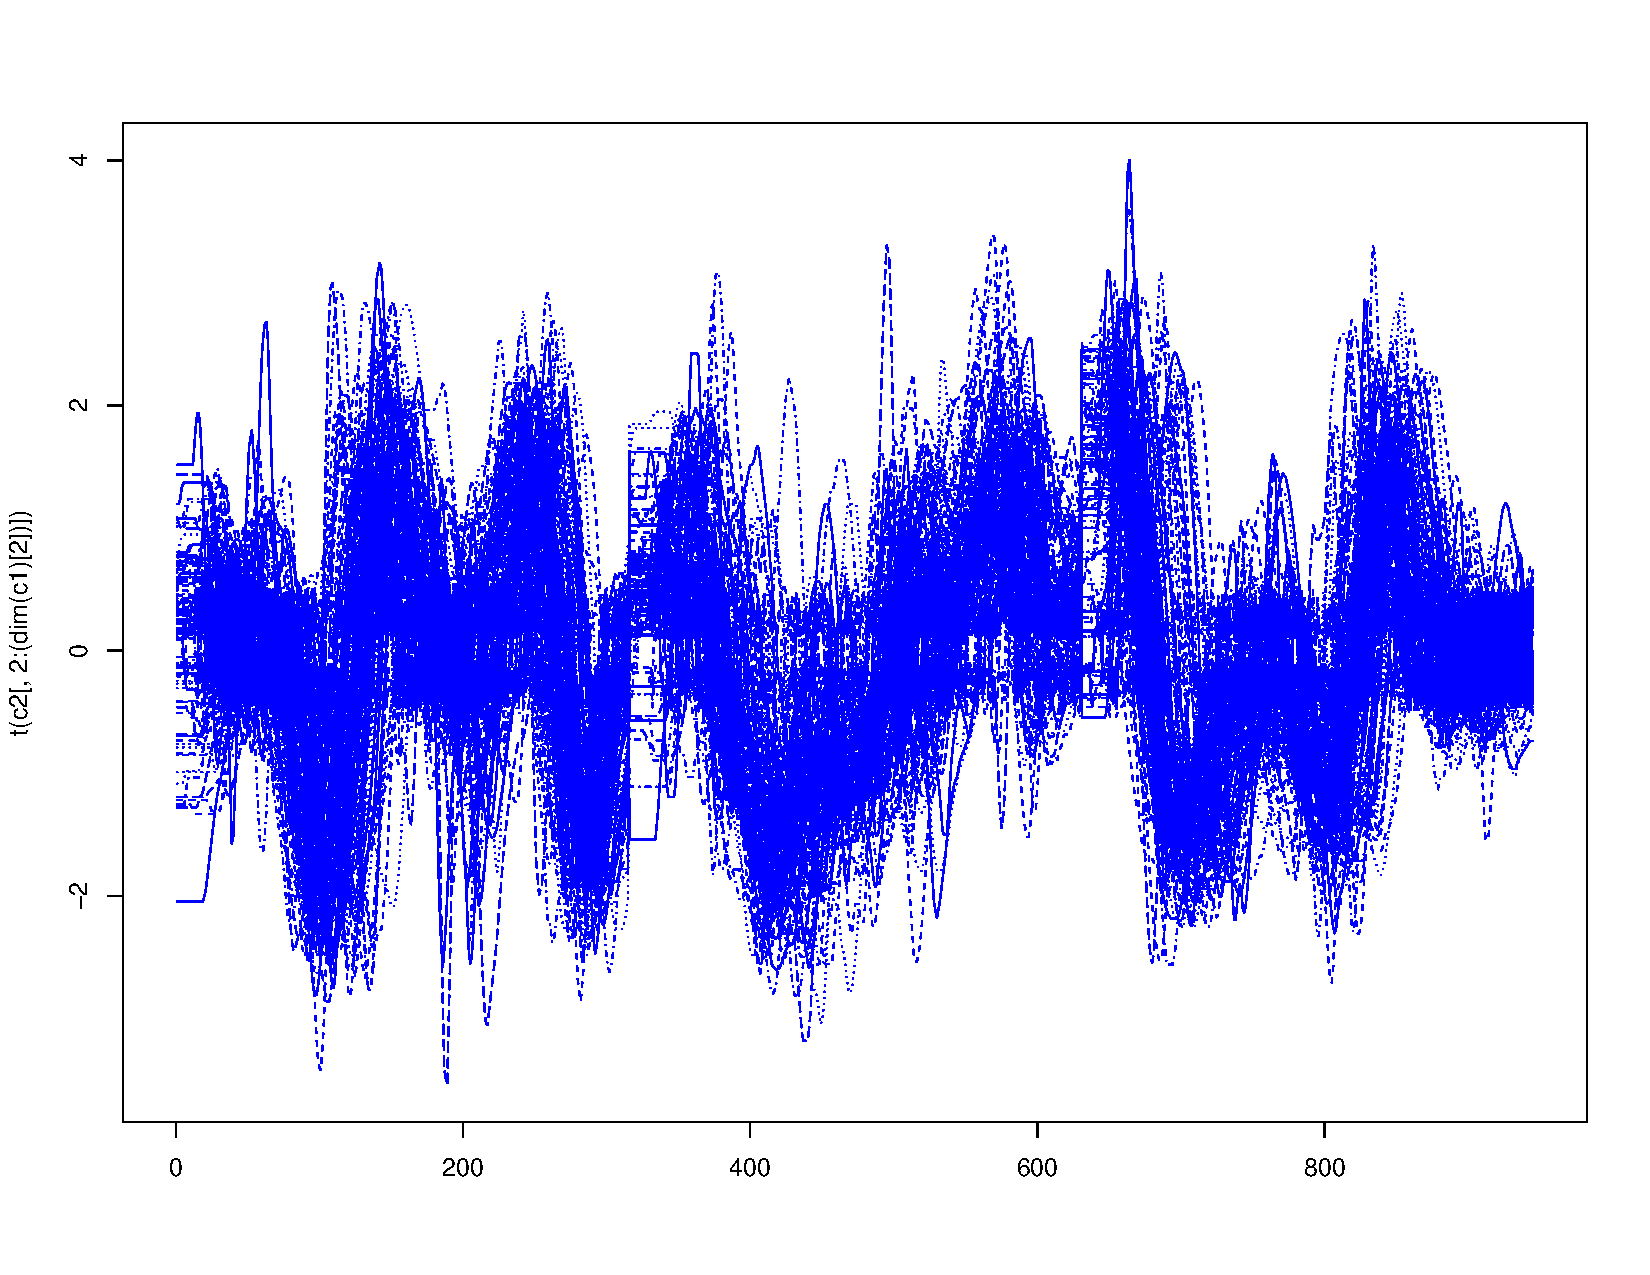
\includegraphics[scale=0.1]{images/c2}
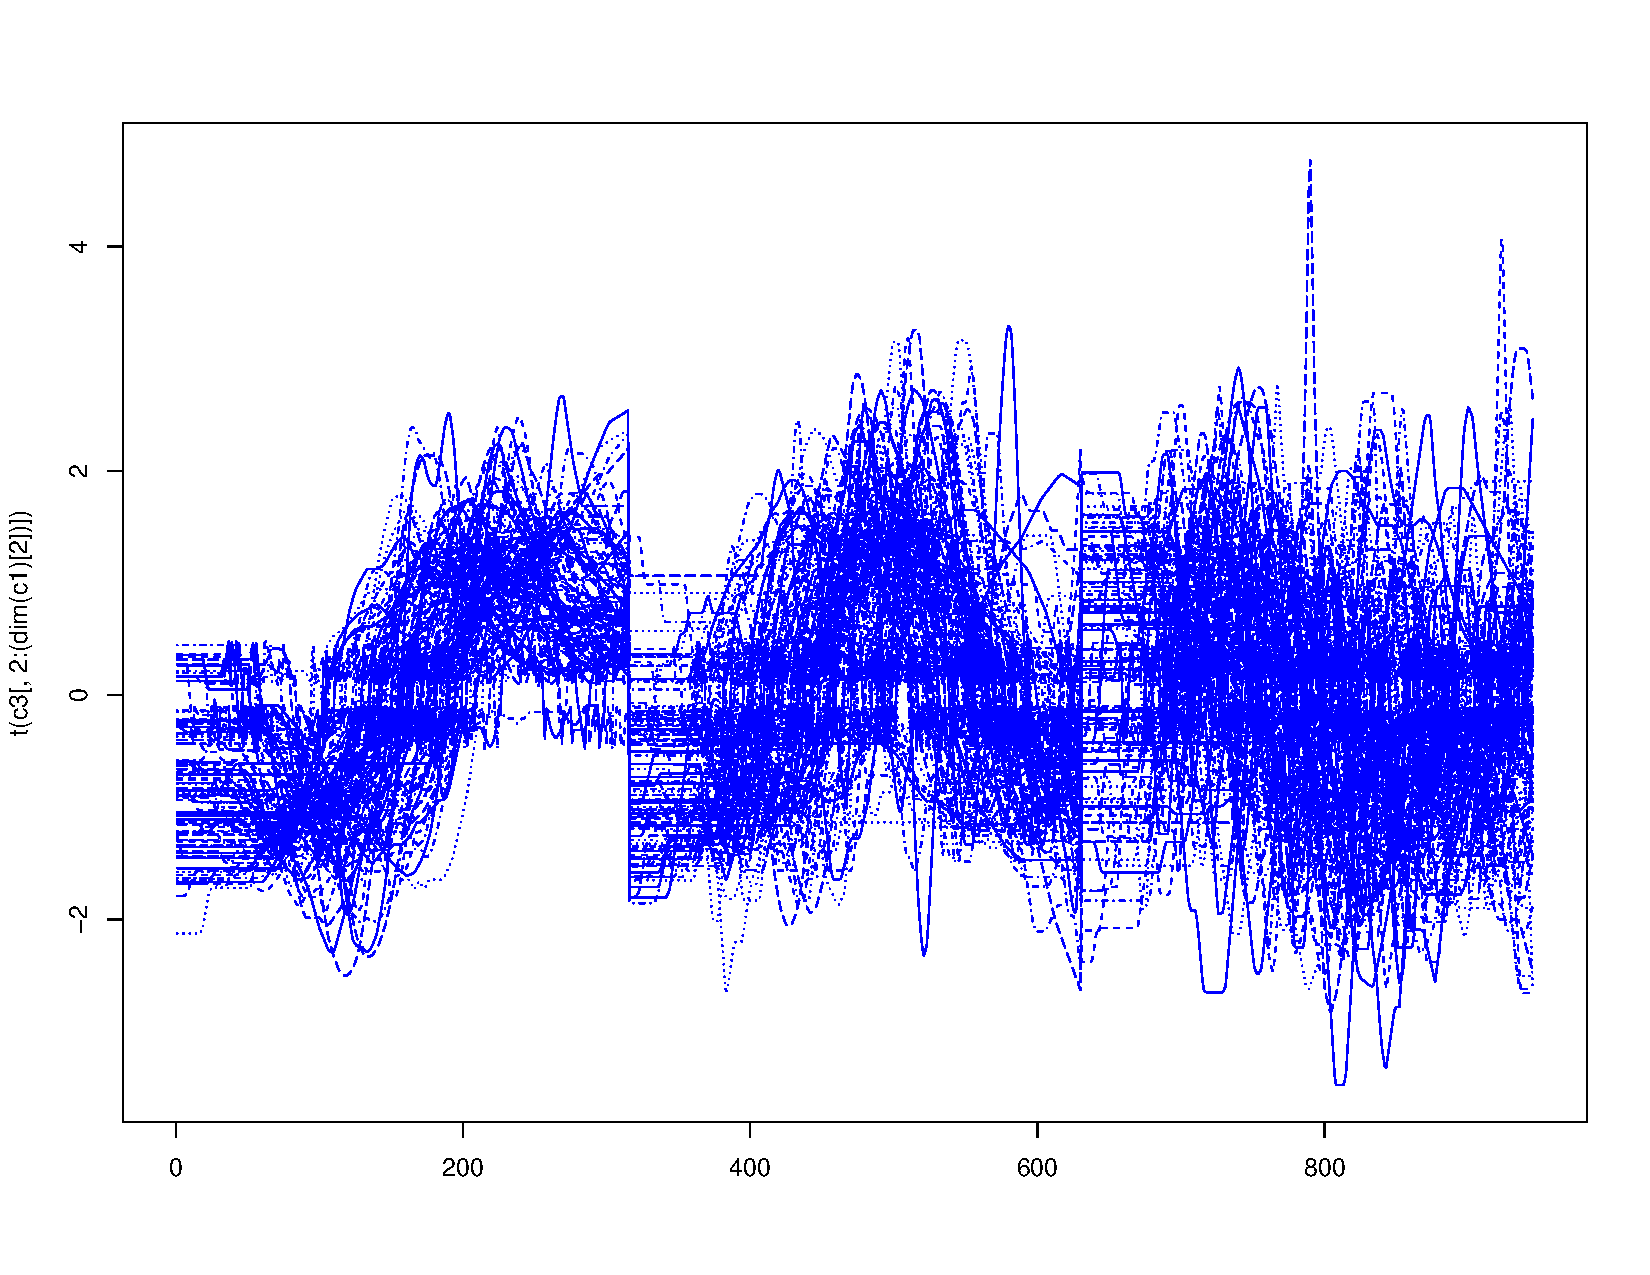
\includegraphics[scale=0.1]{images/c3}
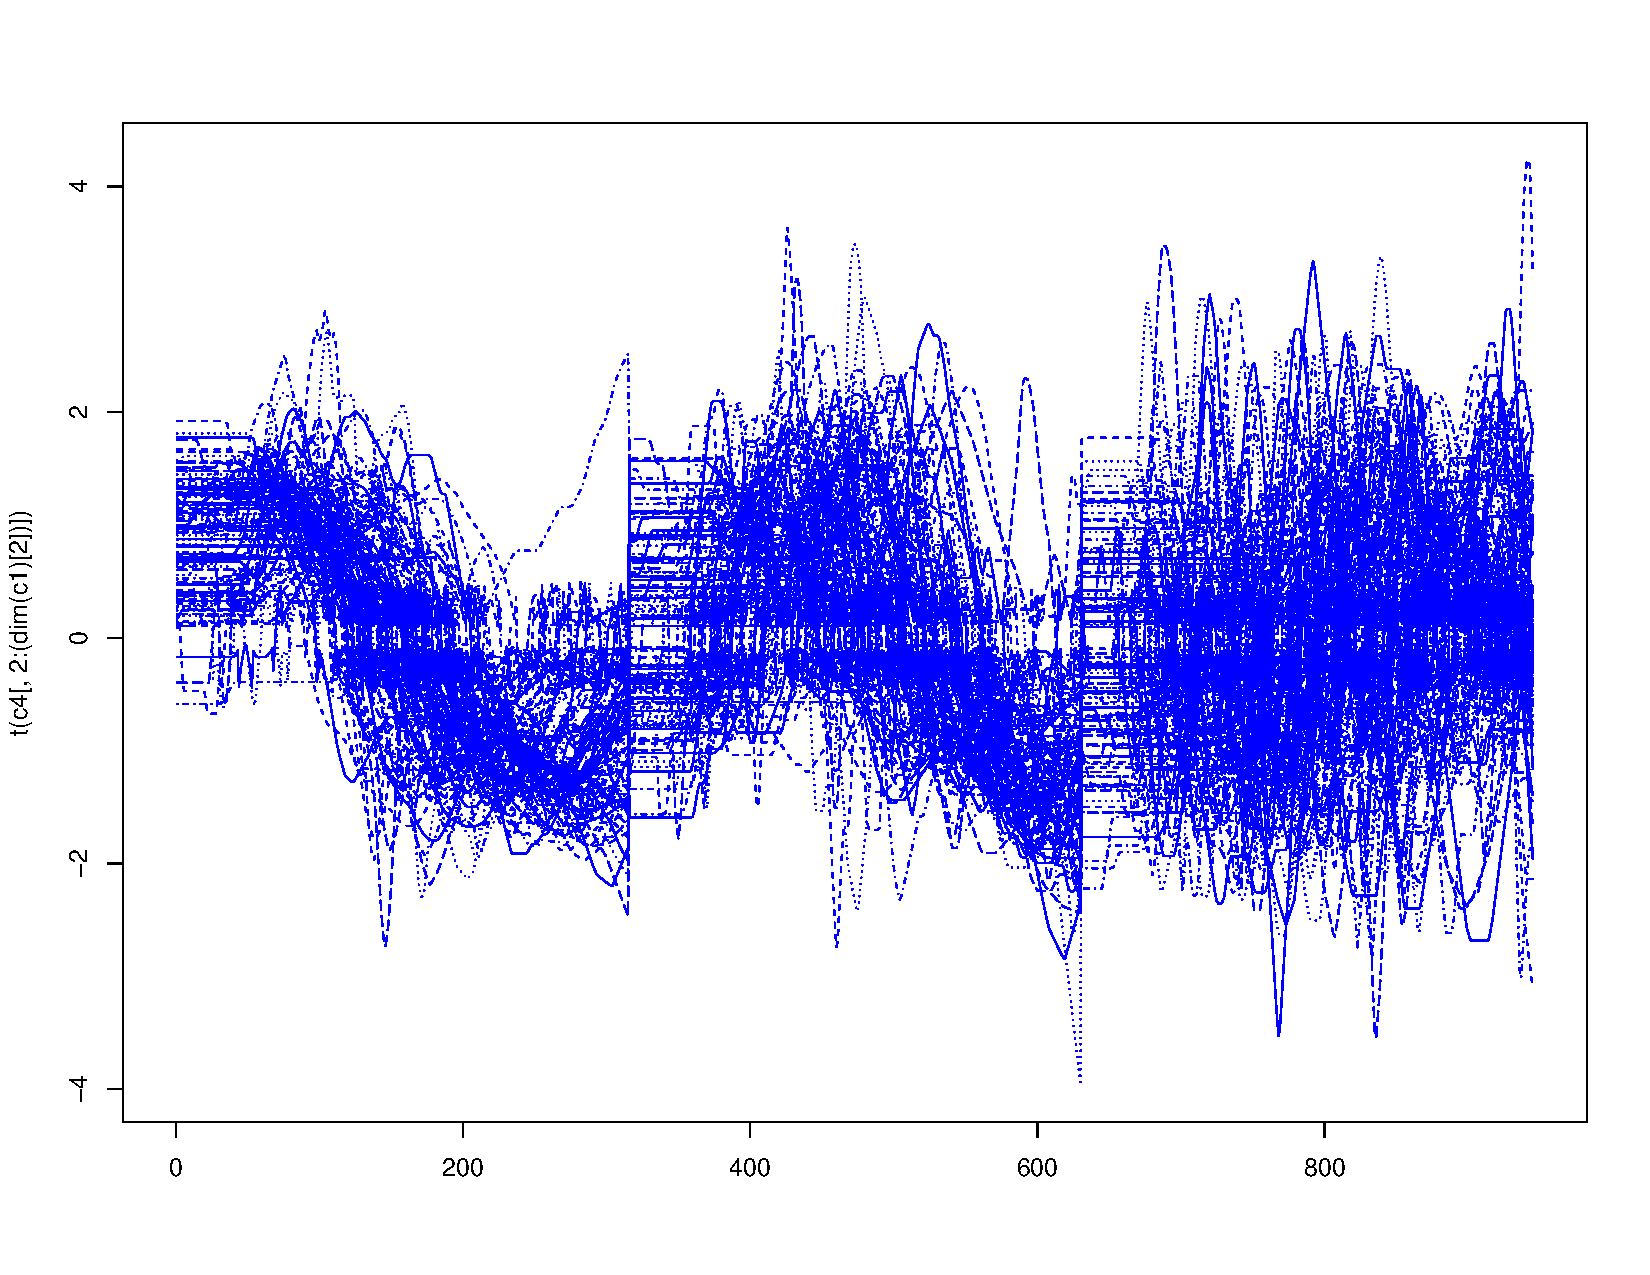
\includegraphics[scale=0.1]{images/c4}
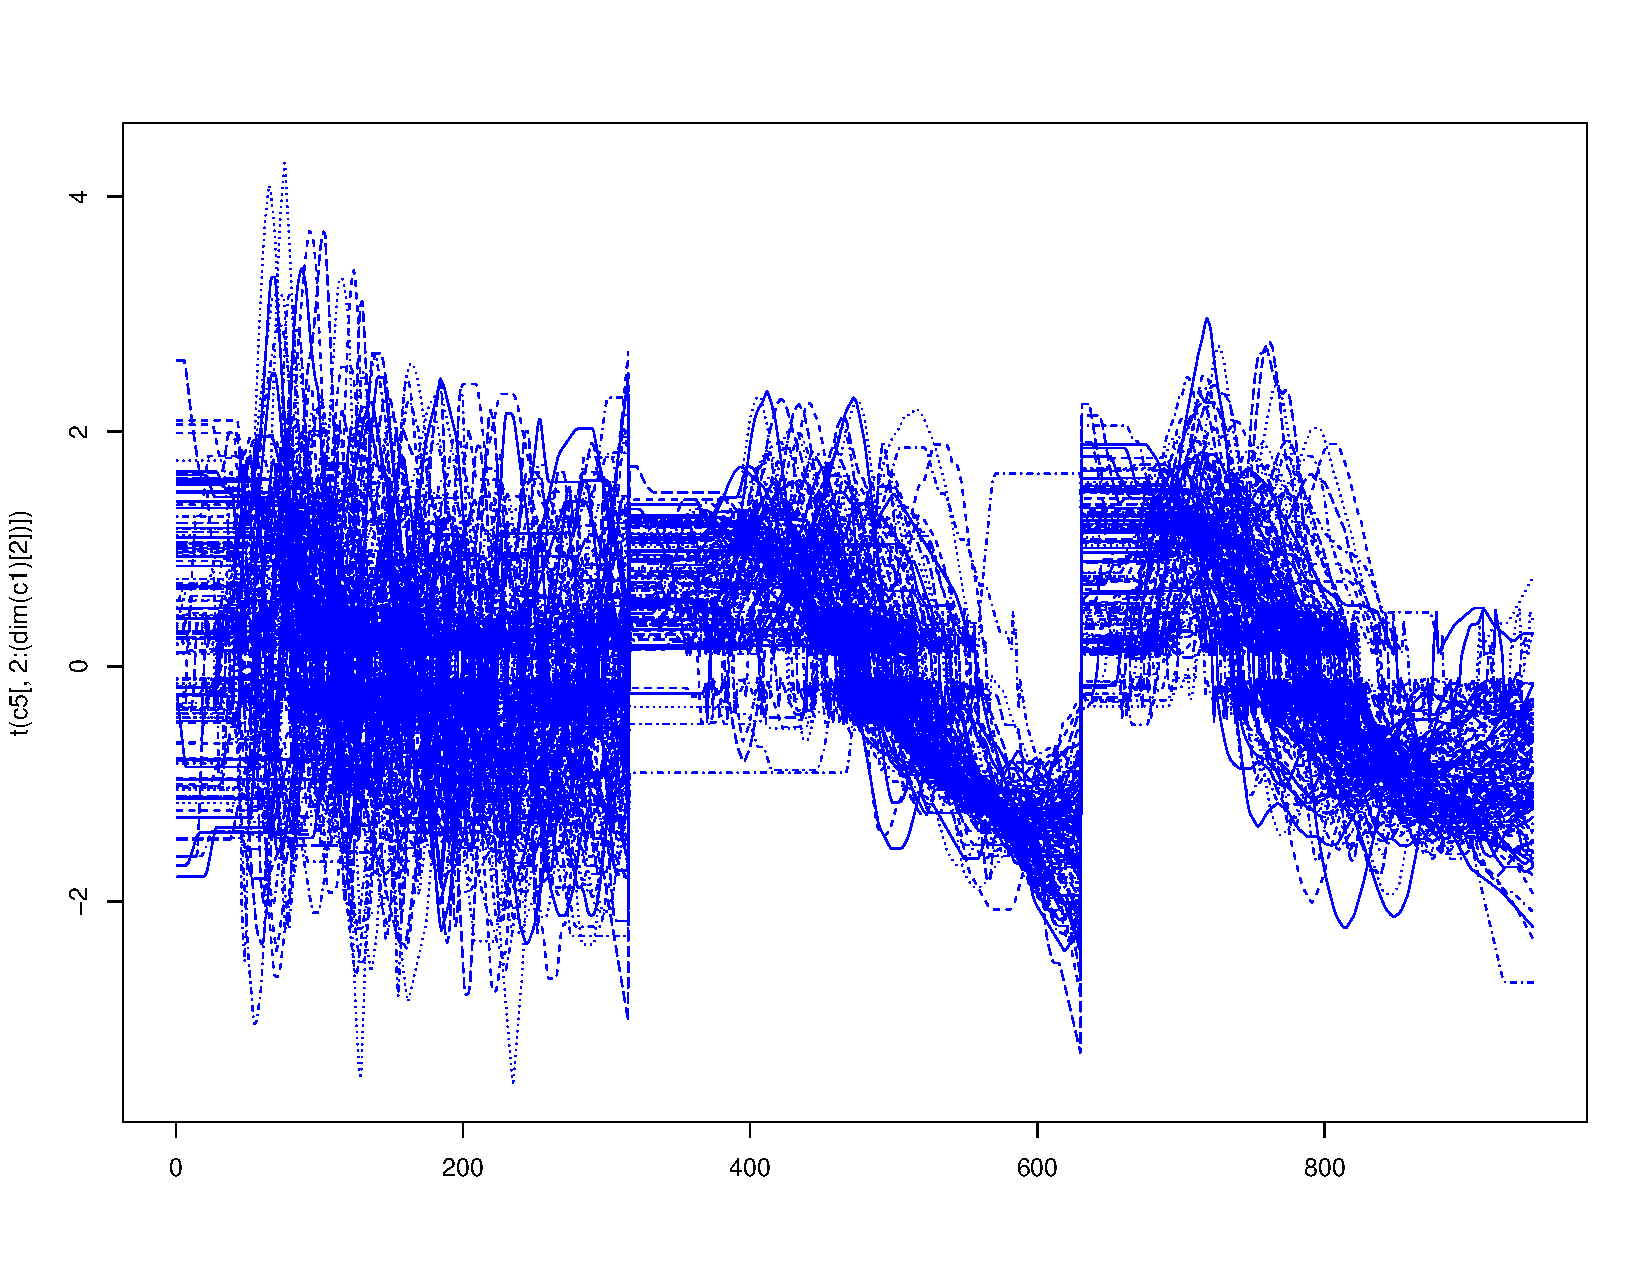
\includegraphics[scale=0.1]{images/c5}
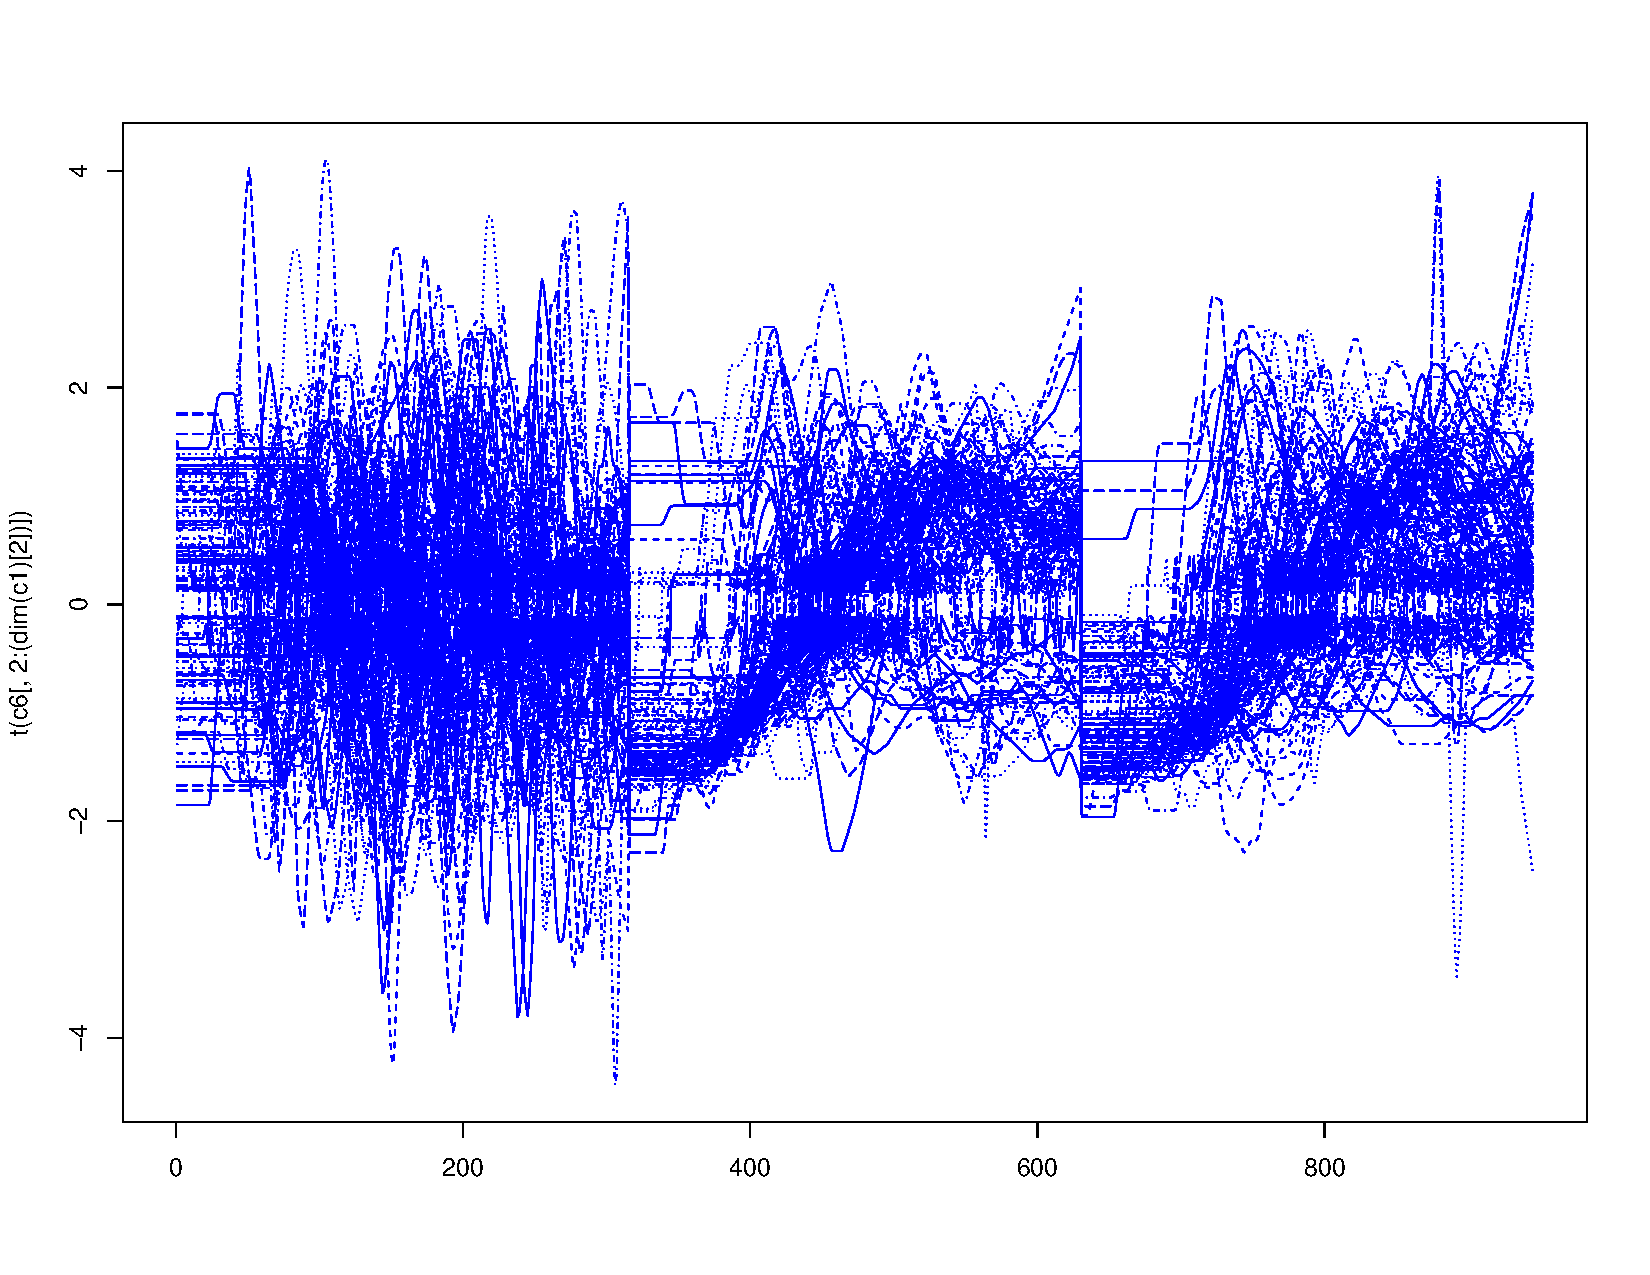
\includegraphics[scale=0.1]{images/c6}
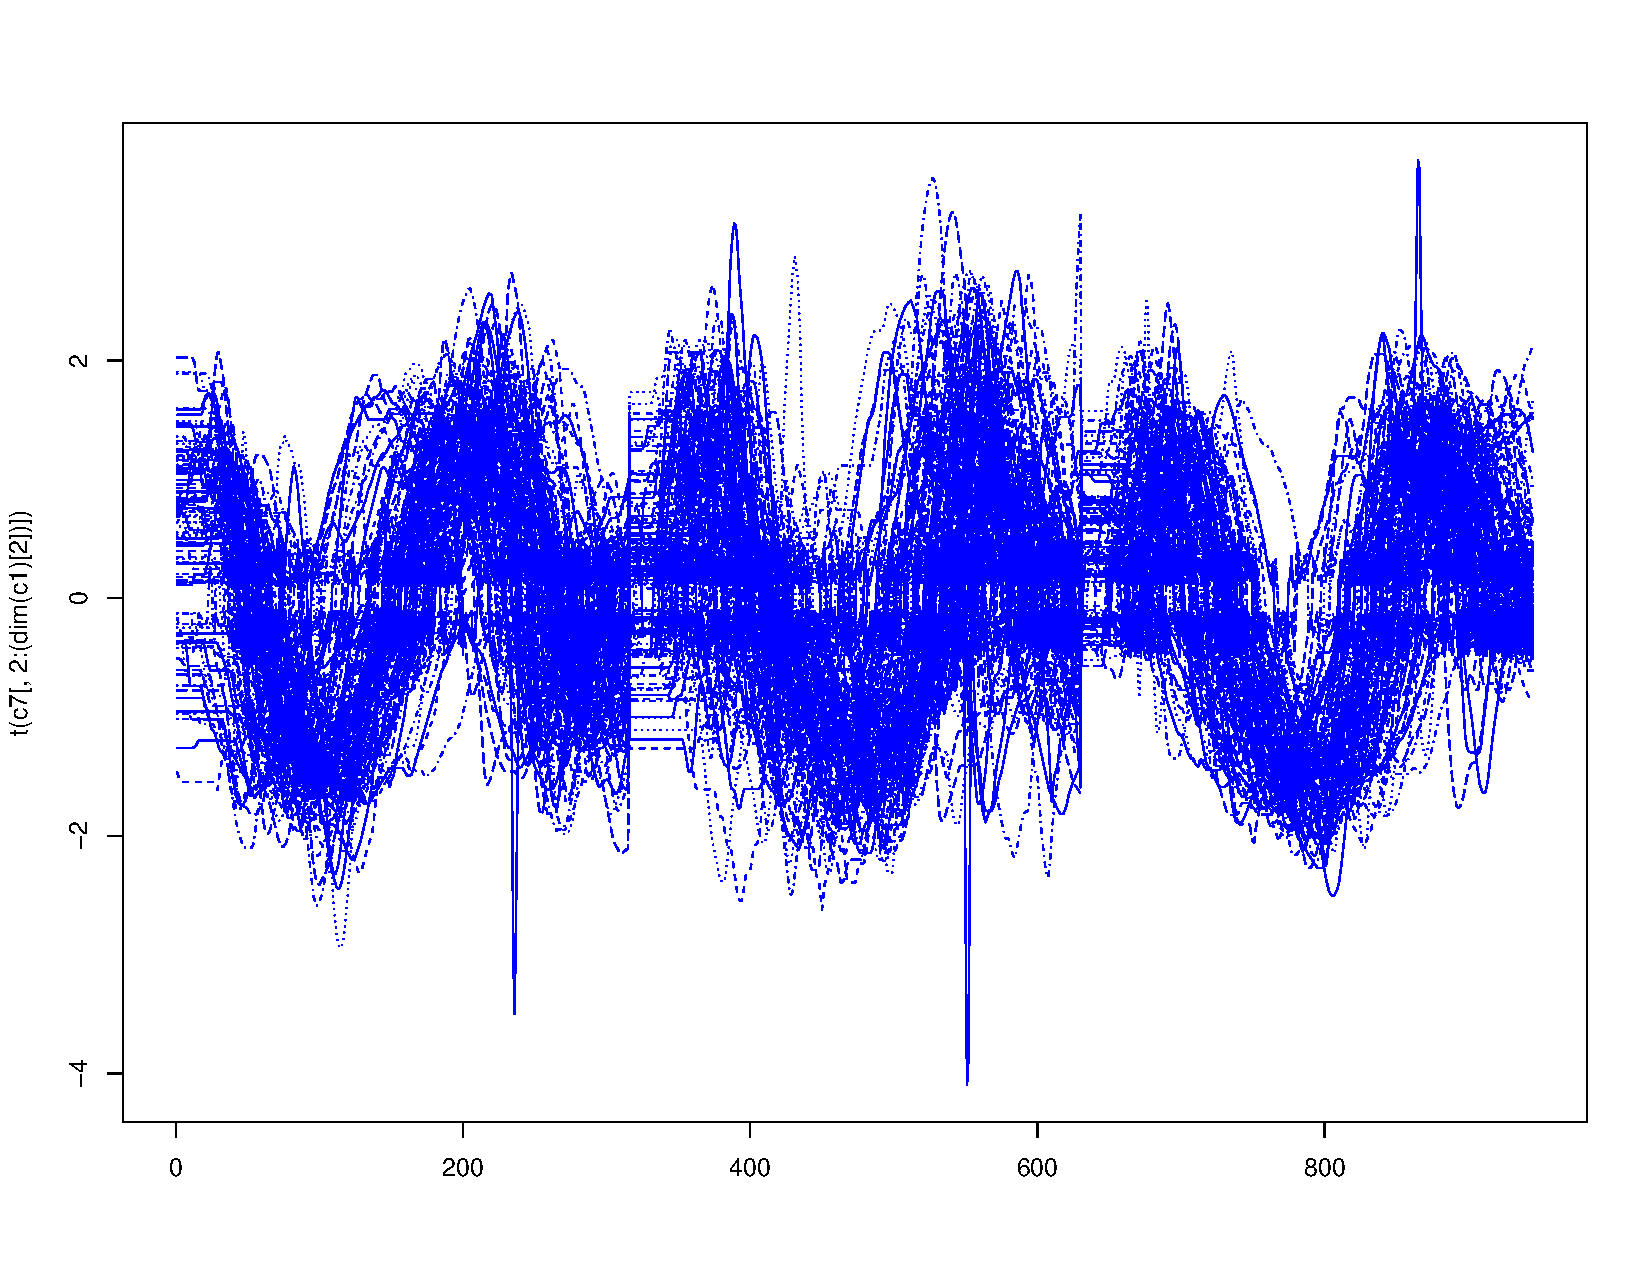
\includegraphics[scale=0.1]{images/c7}
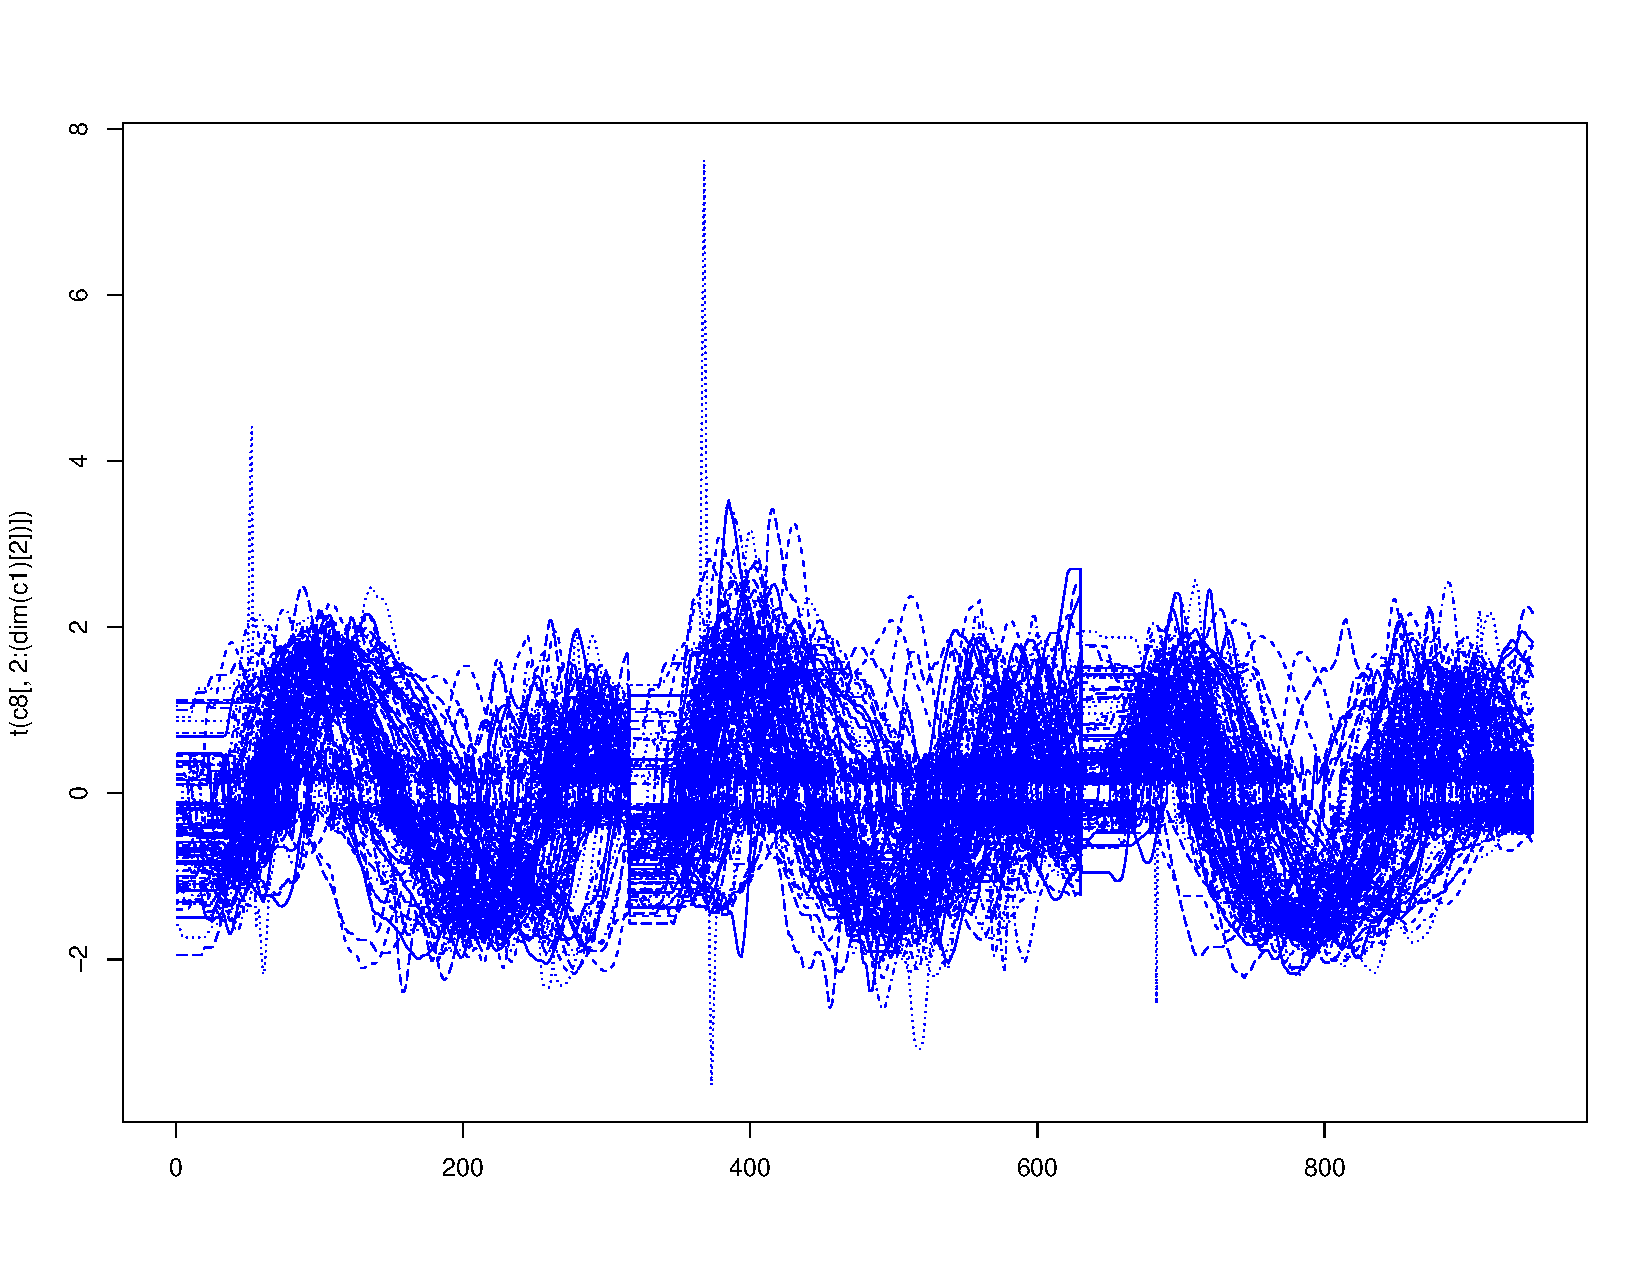
\includegraphics[scale=0.1]{images/c8}

\caption{Eight types of time series corresponding to the vocabulary of 8 gestures.}

\label{geste}
\end{figure}



 Additional experiments are available here \cite{Vanel}. It is possible to consider the internal properties of time series to choose the compression ratio to use with them. However, this approach gives less good results (Appendix \ref{seg}).

\section{Conclusion and perspective}
\label{sec:5}
This chapter deals with the problem of choosing an appropriate number of segments to compress time series with PAA in order to improve the alignment with DTW. In this aim, we proposed a parameter Free heuristic named FDTW, wich approximates the optimal number of segments to use. The experiments showed that,  FDTW increased the quality of alignment of time series especially on synthetic datasets where DTW associated with PAA performed better than any other variant of DTW on a classification task. FDTW was rank 3/37 behind two ensemble classification algorithms COTE and EE. In general, FDTW is faster than Brute force search but run lower than IDDTW. However, FDTW gives a better result than IDDTW on classification task. FDTW also allows reducing the storage space and the processing time of time series while increasing the quality of the alignment of DTW.


 As a perspective, the problem we have dealt with in this chapter could be modeled as a multi-objective optimization problem where one objective function would be compression and the other the classification of time series. 
 
 
Another crucial aspect of time series knowledge discovery is the comparison of time series especially when those time series are uncertain. This aspect will be discussed more in-depth in the next chapter.


%In the next chapter, we will introduce a novel dissimilarity function adapted to the comparison of uncertain time series.


\begin{table}[ht]
\centering
\begin{tabular}{|p{15cm}|}

\hline
\rowcolor{LavenderBlush}
Key points\\
$\bullet$ We proposed a heuristic for time series compression with Piecewise Aggregate  Approximation for classification purpose. \\
\\
$\bullet$ We experimentally showed that in addition to reducing the length and the   processing time of time series, compression can improve the classification of   time series. 
\\
\\
Communications:\\
$-$ Siyou Fotso VS, Mephu-Nguifo E, Vaslin Ph. Parameter Free Piecewise Dynamic  Time Warping. ROADEF, France, Febuary 2017\\
$-$  Siyou Fotso VS, Mephu-Nguifo E, Vaslin Ph. Parameter free piecewise Dynamic Time Warping for time series classification. Time Series workshop at International Conference on Machine Learning, Sydney, Australia, August 2017\\
$-$ Siyou Fotso VS, Mephu Nguifo E, Vaslin Ph. Grasp heuristic for time series compression with piecewise aggregate approximation, Journal RAIRO : Operations Research, accepted. In press.\\
\hline
\end{tabular}
\end{table}